\documentclass[11pt,oneside]{book}
\usepackage[margin=1.2in]{geometry}
\usepackage{setspace}
\usepackage[toc,page]{appendix}
\usepackage[none]{hyphenat} % turn hyphenation off by default
\usepackage{graphicx}
\usepackage[sorting=none]{biblatex}
\usepackage{amsmath}
\usepackage{gensymb}
\usepackage{pgfgantt}
\usepackage{hyperref}
\usepackage{tikz}
\usepackage{float}
\usepackage{caption}
\usepackage{subcaption}
\usepackage{pgfplots}
\usetikzlibrary{matrix}
\hypersetup{
    colorlinks,
    citecolor=black,
    filecolor=black,
    linkcolor=black,
    urlcolor=black
}

\addbibresource{references.bib}

\begin{document}

\frontmatter

\begin{titlepage}

% You need to edit the details here

\begin{center}
{\LARGE University of Sheffield}\\[1.5cm]
\linespread{1.2}\huge {\bfseries Robot Football with the MiRo Robot: Ball Perception and Trajectory Prediction}\\[1.5cm]
\linespread{1}

\includegraphics[width=5cm]{images/tuoslogo.png}\\[1cm]
{\Large Adam Allsebrook}\\[1cm]
{\large \emph{Supervisor:} Alexandr Lucas}\\[1cm]
\large A report submitted in fulfilment of the requirements\\ for the degree of MComp Computer Science\\[0.3cm] 
\textit{in the}\\[0.3cm]
Department of Computer Science\\[2cm]
\today
\end{center}

\end{titlepage}

% -------------------------------------------------------------------
% Declaration
% -------------------------------------------------------------------

\newpage
\chapter*{\Large Declaration}

\setstretch{1.1} % set the line spacing differently if you wish, but this looks good to me. 

All sentences or passages quoted in this report from other people's work have been specifically acknowledged by clear cross-referencing to author, work and page(s). Any illustrations that are not the work of the author of this report have been used with the explicit permission of the originator and are specifically acknowledged. I understand that failure to do this amounts to plagiarism and will be considered grounds for failure in this project and the degree examination as a whole.\\[1cm]

\noindent Name: Adam Allsebrook\\[1mm]
\rule[1em]{25em}{0.5pt}

\chapter*{\Large \center Abstract}

Robot football is a problem in which two opposing teams of robots autonomously play a game of football. Robots are developed not just to compete in these games, but to develop new technologies for the wider field of robotics. A key part of the problem is developing an effective method of ball awareness for the robot.

The aim of this project is to build a ball perception system and trajectory prediction for the MiRo robot. This involves creating a computer vision algorithm which is robust to a very dynamic world state, as well as accurately modelling the trajectory of the ball, to allow players to quickly and efficiently intercept it. 

The project successfully develops an efficient ball detection algorithm using non-neural methods including a circular Hough transform and a support-vector machine classifier with a histogram of oriented gradients feature descriptor, as well as overcoming problems with image space to world space conversion. 

% -------------------------------------------------------------------
% TOC etc
% -------------------------------------------------------------------

\tableofcontents
\listoffigures
\listoftables

\setstretch{1.1} 

\mainmatter

\chapter{Introduction}

\section{Project Aims and Motivation}

The project aims to build a ball perception system, to be a component of a complete football playing  robot. The system will be made for the MiRo robot which has forward-facing stereo cameras that can be used for ball detection, however its limited processing power is a factor that will limit the techniques that can be used to achieve this. 

There are three key problems that the project will tackle; measuring ball position, measuring ball velocity and predicting ball trajectory. 

The ball position can be detected using the cameras, however it must be measured in world space to be useful for decision making. Therefore an world space conversion is required as well as a computer vision algorithm. This algorithm should be reasonably accurate while being efficient enough to run in real time.

The ball velocity can be estimated using recent observed ball positions, however noise in these observations should be expected. 

A prediction for the ball trajectory is necessary for planning a route to intercept the ball. 

\section{RoboCup}

In 1993 a group of Japanese researchers decided to start a robot football league, and after receiving great support from researchers across the world the league was made international, and named the Robot World Cup initiative, or RoboCup for short. Four years later the first ever RoboCup competition was held in Japan. 

The tournament is held annually, having teams compete in 5 types of football leagues: humanoid, standard platform, middle size, small size and simulation. RoboCup also has some leagues for problems outside of football: rescue, home and industrial.

Since its conception, the goal of RoboCup has been the following: "By the middle of the 21st century, a team of fully autonomous humanoid robot soccer players shall win a soccer game, complying with the official rules of FIFA, against the winner of the most recent World Cup." This makes RoboCup a landmark project - the accomplishment of this goal would be a landmark in the history of mankind. RoboCup is also a standard problem - technologies developed to achieve its goal will be useful in the area of AI and robotics.

\section{MiRo}

MiRo is an animal-like robot developed by Consequential Robotics for education and research purposes. MiRo excels in its social behaviour, with numerous touch sensors around its body and 11 degrees of freedom allowing believable animal-like movement. However MiRo also has all of the necessary features to be able to play football. 

It has stereo cameras able to capture images in 720p. Each camera has a 120\degree horizontal field of view with an overlap slightly over 60\degree meaning that they have a combined horizontal field of view of nearly 120\degree. MiRo can move using a differential drive platform that gives a maximum speed of 400mm/sec. The biggest limitation of the robot is its onboard computer, a Raspberry Pi 3B+ containing a 1.4GHz 64-bit quad-core processor. 

\begin{figure}[H]
    \centering
    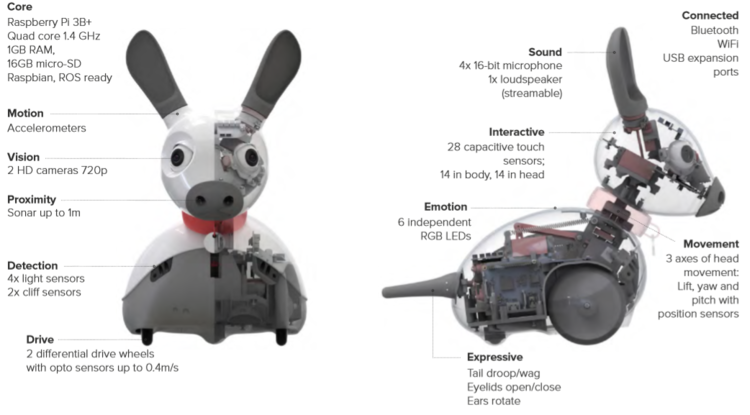
\includegraphics[width=12cm]{images/miro-specs.png}
    \caption{Full specifications of the MiRo robot}
    \label{fig:miro specs}
    Source: \url{https://www.miro-e.com/robot}
\end{figure}

\section{Computer Vision}

Computer vision is a field of artificial intelligence which is concerned with the extraction of information from digital images. It has many sub-domains, such as object recognition or identification, but the perception of a ball in an image falls into object detection. 

Object detection is a technique that involves finding instances of a specific class in an image. The various methods of object detection can be classified into two approaches, neural and non-neural. For non-neural techniques, a feature vector must be obtained from the image, which must then be evaluated by a classifier. Neural techniques are able to do object detection without needing to defining features. They can be more powerful than non-neural methods, however they are more computationally expensive to train and to run.

\section{Motion Planning}

Motion planning is the problem of finding a valid path so that a robot moves from some initial position to a goal, avoiding any obstacles along the way. Bruce\cite{Bruce2006} outlines some different categories of dynamics in motion planning problems. The first is agent and domain dynamics. Agent dynamics refers to the effects of physics on the agent itself, for example the kinematic constraints on the motion of the agent. Conversely domain dynamics involves changes to the problem instance over time, for example changes in the environment or goal state.

Another way of categorising dynamics is into predictable and unpredictable dynamics. Predictable dynamics involve variables that can accurately be modelled, such as using the physics of acceleration and velocity. Unpredictable dynamics relate to aspects that cannot be modelled, for example actions taken by other agents, humans or random events.

Bruce also categorises dynamics into local and global dynamics, describing that effect the local and non-local areas to the agent respectively.

This project only aims to tackle the predictable domain dynamics of building an accurate model for the movement of the goal state (i.e. the ball).

\section{Overview of the Report}

Chapter \ref{chapter: 2} gives an overview of relevant work that has already been completed, primarily by teams competing in previous iterations of RoboCup. This includes methods for estimating ball position and velocity, as well as predicting ball trajectory. 

Chapter \ref{chapter: 3} outlines the objectives that the project aims to achieve, elaborating on each point and giving detail on how each part of the system will be evaluated. 

Chapter \ref{chapter: 4} provides detail on the design of the project. This starts with a description of the tools that are used to develop the system, and then goes on to break down and justify each decision that had to be made regarding the design of each part of the system. 

Chapter \ref{chapter: 5} goes into detail about the notable algorithms that were developed, including the circular Hough transform, support-vector machine classifier and image space to world space conversion. 

Chapter \ref{chapter: 6} presents the results showing the performance of each part of the system, and discusses how successfully each objective was met as well as suggesting some areas for which future work on the system could be completed. 

Chapter \ref{chapter: 7} brings the project to a close, summarising what has been achieved.
\chapter{Literature Review}
\label{chapter: 2}

This chapter provides an in depth look into technical solutions for the problems that the project will tackle, divided into three key areas: ball position, ball velocity and ball trajectory. The primary source for this research is from papers written by past participants in the RoboCup competition. 

\section{Measuring Ball Position}

\subsection{Camera Calibration}

Camera calibration (specifically geometric camera calibration) is the process of estimating the parameters of a camera to remove distortions from the images it captures. A camera has two types of parameters that can be estimated: intrinsic and extrinsic. Hartley and Zisserman \cite{Hartley2004} describe these parameters.

Extrinsic parameters define the transformation between 3D world coordinates and 3D camera coordinates. This includes a rotation $R$ and a translation $T$. 

The intrinsic parameters for a camera are its focal length in pixels $(f_x, f_y)$, its optical centre in pixels $(c_x, c_y)$ and the skew coefficient between the x and y axes $s$, although this is often zero. The parameters can be summarised in the camera intrinsic matrix $K$:

\[ K = 
\begin{bmatrix}
f_x & s & c_x\\
0 & f_y & c_x\\
0 & 0 & 1
\end{bmatrix}
\]

The output of a camera may also be affected by lens distortion. The first type of lens distortion is radial distortion which can cause straight lines to appear curved. It can be represented as follows:

\[ x_{distorted} = x(1+k_1 r^2 + k_2 r^4 + k_3 r^6) \]
\[ y_{distorted} = y(1+k_1 r^2 + k_2 r^4 + k_3 r^6) \]

\noindent where $x, y$ are the undistorted pixel positions, $k_1, k_2, k_3$ are the radial distortion coefficients and $r^2 = x^2 + y^2$.

The other type of lens distortion is tangential distortion which causes some parts of the image to appear closer than they should be. It can be represented as follows: 

\[ x_{distorted} = x + [2 p_1 x y + p_2(r^2 + 2 x^2)] \]
\[ y_{distorted} = y +[p_1 (r^2 + 2 y^2) + 2 p_2 x y] \]

\noindent where $x, y$ are the undistorted pixel positions, $p_1, p_2$ are the tangential distortion coefficients and $r^2 = x^2 + y^2$.

The five parameters that need to be estimated are given by:

\[ \text{Distortion coefficients} = (k_1, k_2, p_1, p_2, k_3) \] 

\nocite{Zhang2000}
\nocite{Heikkila1997}
\nocite{Ling2019}

\subsection{Non-Neural Object Detection}

Object detection is a type of computer vision problem that attempts to find instances of an object class in an image. In this case the problem is specific to finding the location of a single ball in an image. One approach to this problem is the non-neural approach, in which various types of algorithms must be combined to find these instances. 

Feature extraction algorithms aim to reduce the complexity of some data by picking out only the relevant features. In the field of computer vision this involves finding relevant areas of interest in an image. 

Feature descriptors take an image and output a feature vector, which is a representation of the original image in a format that can more easily be processed by models such as classifiers. 

A classifier is a model that can assign an output value to a given input feature vector. This project only looks at binary classifiers, in which the output is either true or false. Many classifiers are trained using supervised learning, which is a type of machine learning algorithm that learns how to map the input to output from a dataset of labelled input-output pairs. 

\subsubsection{Circular Hough Transform}

The Hough transform is a feature extraction algorithm originally designed to detect lines in an image, which has since been extended to detect arbitrary shapes. To identify the position of a ball, the circular Hough transform is useful. The first step is to apply an edge detection operator, for example the Sobel or Canny edge detectors. Next the parameter space must be decided. 

\[ r^2 = (x-a)^2 + (y-b)^2 \]

For a circle with a known radius \textit{r}, the search for the centre \textit{(a, b)} can be conducted in 2D parameter space. If the radius is unknown a 3D parameter space is required as the radius must also be searched for. Now the voting procedure can take place, resulting in an accumulator where each point in the parameter space is assigned a value by the Hough transform. The coordinates of the peaks in the accumulator correspond to the attributes of the circles found in the image \cite{ribeiro2009}.

The performance of the algorithm could be improved by first applying a colour segmentation to the image \cite{jonker}. False positives could be removed by validating the results. A distance-dependant threshold could be introduced, so closer candidates require a larger value for their local maximum to be included. Another validation could be checking that the sum of all floor coloured pixels in a bounding box drawn around the candidate is not too large \cite{cambada}.

\subsubsection{Colour Image Segmentation}

Image segmentation is the process of breaking down an image into various segments to make analysis easier. Colour segmentation uses the colour information of the image to create these segments. First the colour space must be chosen, for example RGB, HSV or YUV. Colour classes are then chosen as ranges inside this colour space and stored in a lookup table. HSV is the easiest to calibrate colour classes for, due to the colour information being limited to only the hue channel. Colour classes can be calibrated manually by a human, although this is tedious and not robust to changes in lighting. Automatic on-line calibration \cite{Guerrero2008} could be used instead to provide better results.

A simple method of segmenting the image is to calculate the colour class of each pixel individually according to the lookup table, but a more sophisticated technique such as colour region growing \cite{Gunnarsson2006} can achieve better results.

\subsubsection{K-Means Clustering}

K-means clustering aims to cluster data into k clusters, where each data point belongs to the cluster with the nearest mean. The problem is NP-hard but Hartigan and Wong\cite{Hartigan1979} present an efficient algorithm, that aims to find local optima rather than a perfect solution.

In image processing, k-means clustering can be used to find what colours are in an image, and which colours are the most dominant. The most important parameter is k, too few clusters could mean that different colours are included in the same cluster whereas too many clusters could mean that one colours is separated into multiple clusters.

\begin{figure}[ht]
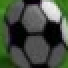
\includegraphics[width=3cm]{images/kmeans_ball.png}

\includegraphics[width=3cm]{images/kmeans_palette.png}
\centering
\caption{An example of using k-means clustering to find the dominant colours in an image}
\end{figure}

\subsubsection{Histogram of Oriented Gradients}

The histogram of oriented gradients (HOG) is a method of feature description, meaning that it summarises interesting information about an image into a feature vector. The algorithm breaks the image down into smaller cells and analyses the edge directions in these cells, building a histogram of gradient directions. The implementation of the algorithm as described by Dalal and Triggs \cite{Dalal2005} is outlined below:

\begin{enumerate}
    \item Gradient Computation
    
    Dalal and Triggs discuss preprocessing in the form of gamma/ colour normalisation, but find that it has little effect, possibly due to the normalisation in later steps achieving the same results. The first step is therefore to calculate the gradient values in both the horizontal and vertical directions. Dalal and Triggs suggest to use the following filter kernels:
    \[ [-1, 0, 1] \text{ and } [-1, 0, 1]^T \]
    
    
    \begin{figure}[H]
        \caption{An example of gradient computation}
        \centering
        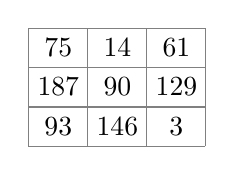
\begin{tikzpicture}
        \draw[xstep=0.75cm,ystep=0.5,color=gray] (0,0) grid (2.25,1.5);
        \matrix[matrix of nodes,
        inner sep=0pt,
        anchor=south west,
        nodes={inner sep=0pt,text width=.75cm,align=center,minimum height=.5cm}
        ]{
        75 & 14 & 61 \\
        187 & 90 & 129 \\
        93 & 146 & 3 \\
        };
        \end{tikzpicture}
        
        The gradients at the centre pixel are:
        
        Gradient in x direction = $129 - 187 = -58$
        
        Gradient in y direction = $146 - 14 = 132$
    \end{figure}
    
    
    \item Spatial/ Orientation Binning
    
    The next step is to compile these gradients into a histogram. The image is broken down into cells, each of which has a set of orientation bins. These bins are evenly spaced over the range 0\degree - 180\degree for an unsigned gradient. Dalal and Triggs find that using any more than 9 bins has little difference on performance. Each pixel calculates a weighted vote using the orientation and magnitude of the gradient at that point, which is accumulated into the orientation bins for that cell.
    
    \begin{figure}[H]
        \caption{An example for HOG orientation binning}
        \centering
        The orientation at the centre pixel can be calculated by $atan(\frac{132}{-58}) = -66.28\degree$
        
        As an unsigned orientation $-66.28\degree + 180\degree = 133.72\degree$
        
        Assuming a magnitude of 100, this orientation is inserted into a blank set of orientation bins.
        
        \[100 * \frac{13.72}{20} = 68.6, 100 * \frac{6.28}{20} = 31.4 \]
        
        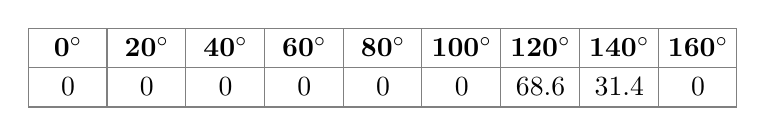
\begin{tikzpicture}
        \draw[xstep=1cm,ystep=0.5,color=gray] (0,0) grid (9,1);
        \matrix[matrix of nodes,
        inner sep=0pt,
        anchor=south west,
        nodes={inner sep=0pt,text width=1cm,align=center,minimum height=.5cm}
        ]{
         \textbf{0\degree} & \textbf{20\degree} & \textbf{40\degree} & \textbf{60\degree} & \textbf{80\degree} & \textbf{100\degree} & \textbf{120\degree} & \textbf{140\degree} & \textbf{160\degree} \\
         0 & 0 & 0 & 0 & 0 & 0 & 68.6 & 31.4 & 0 \\
        };
        \end{tikzpicture}
    \end{figure}
    
    \item Normalisation and Descriptor Blocks
    
    Local normalisation is used to reduce the effect of variations in illumination and contrast. Cells are grouped into larger blocks, which typically overlap. The normalisation is then calculated over these blocks. Dalal and Triggs evaluate two classes of block geometries, rectangular (R-HOG) and circular (C-HOG). They found that the optimal configuration for R-HOG is for blocks to be made up of 4 cells in a square. 
    
    Dalal and Triggs describe four block normalisation methods. Let \textbf{v} be the unnormalised descriptor vector, $||\textbf{v}||_k$ be its \textit{k}-norm  for \textit{k} = 1,2, and $\epsilon$ be a small constant. 
    \[ \text{L2-norm: } \textbf{v} = \frac{\textbf{v}}{\sqrt{||\textbf{v}||^2_2 + \epsilon^2}} \]
    L2-Hys: L2-norm followed by clipping (limiting the maximum values of \textbf{v} to 0.2) and renormalising
    \[ \text{L1-norm: } \textbf{v} = \frac{\textbf{v}}{||\textbf{v}_1|| + \epsilon} \]
    \[ \text{L1-sqrt: } \textbf{v} = \sqrt{\frac{\textbf{v}}{||\textbf{v}_1|| + \epsilon}} \]
    
\end{enumerate}


\begin{figure}[ht]
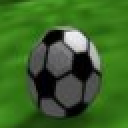
\includegraphics[width=3cm]{images/hog_ball.png}
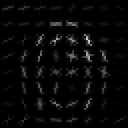
\includegraphics[width=3cm]{images/hog.png}
\centering
\caption{A visualisation of the HOG descriptor}
\end{figure}

Farazi et al. \cite{Farazi2016} use a HOG descriptor for a cascade classifier, trained using the AdaBoost technique to reject false positives from a list of ball candidates. As the HOG descriptor is not rotation invariant, for each positive sample in their dataset they add samples rotated by 10\degree, 20\degree and mirrored horizontally. The rotations are limited to this amount to allow the classifier to learn the shadow under the ball.

\subsubsection{Support-Vector Machine Classifier}

The support-vector machine is a supervised learning model for the two-group classification problem. The algorithm was developed by Cortes and Vapnik\cite{Cortes1995}. The goal of the machine is to find the hyperplane that separates the two classes while having the largest distance to the nearest data point of either class. However, there is often not a linear solution in the original dimensional space. To solve this, the data is be mapped to a higher-dimensional space, for which a linear solution does exist. This process is optimised by ensuring that the dot product can be used to transform hyperplanes between these dimensional spaces.

\begin{figure}[H]
    \centering
    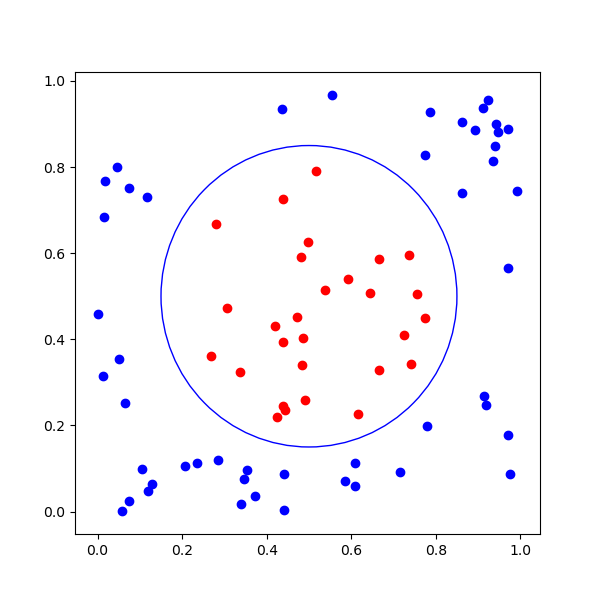
\includegraphics[width=5cm]{images/svm1.png}
    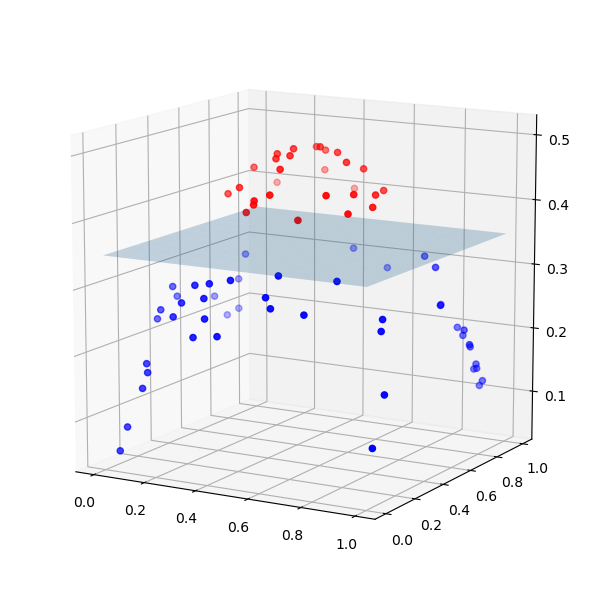
\includegraphics[width=5cm]{images/svm2.png}
    \caption{An illustration of an SVM mapping to a higher dimensional space}
    \centering
\end{figure}

Menashe et al. \cite{Menashe2017} compare the SVM to simple deep neural network (DNN) models for ball classification in RoboCup. They find that both methods have high accuracy, although the DNNs have a higher recall. The generalisation of the models is also tested, with the SVM producing much worse results for a different dataset. This highlights the importance of training the classifier on a dataset which is representative of the situations that could occur in a real game. 

\subsubsection{Ensemble Learning and AdaBoost}

In ensemble learning, a classifier is formed by combining multiple less accurate algorithms. An ensemble is guaranteed to be more accurate than any of its individual members if each classifier is accurate (better than random guessing) and diverse (makes different errors on new data points). Dietterich\cite{Dietterich2000} compares various methods of constructing ensembles, and concludes that AdaBoost is the most effective.

AdaBoost (short for adaptive boosting) is a type of boosting algorithm introduced by Freund and Schapire\cite{Freund1996}. The algorithm builds an ensemble classifier by training subsequent models to correct the mistakes of previous model. This is achieved by assigning a weight to each sample in the training data, and increasing these weights for samples which have previously been misclassified.

\subsection{Neural Object Detection}

The neural approach to object detection produces results directly from an input image, without any intervening algorithms, at the cost of increased computational complexity. The primary method for this the the convolutional neural network.

\subsubsection{Convolutional Neural Network}

A artificial neural network (ANN) is a computational model that is made up of a series of connected neurons, much like the human brain. Traditional ANNs are not suitable for image processing due to the computational complexity of the number of connections required. A convolutional neural network (CNN) is a class of ANN that uses convolutional layers to reduce the number of connections between layers, thus making them effective in processing images.

Convolutional layers learn kernels as parameters. Kernels are matrices that are convolved across the width and height of the input to produce an activation map. The activation maps for each kernel are stacked together to produce the layer's output. Convolutional layers have three hyperparameters, depth, stride and padding. The depth refers to the number of neurons in a layer that connect to the same region of the input. The stride sets how many pixels kernels should move at a time, and can cause overlapping between regions. Padding controls how many pixels should be added to the border of the output, this is commonly used to preserve the size exact size of the input.

Pooling layers are used for dimensionality reduction, decreasing the computation power needed to process the layer. The most common type is max pooling, where the image is broken down into smaller regions and only the maximum value is taken from each. 

Fully connected layers are used at the end of the network for classification \cite{cnn}.

In RoboCup various approaches have been taken for classification of the ball position. One method is to break the image down into smaller "patches" and evaluate each patch between two classes: ball or no ball. This has the advantage a large quantity of training data is easier to produce, however each patch does not have any further context about the image which can make classification more difficult \cite{Gabel2018}. Alternatively the network could be trained to estimate a 2D normal distribution of the ball's position, where the distortion of the distribution also gives an idea of how noisy the image is \cite{Speck2016}. Another method is to have the output be a low resolution heatmap of the original image, which can achieve pixel level accuracy of the ball's position \cite{Speck2018}.

\nocite{Kukleva2019}
\nocite{Teimouri2019}

\subsection{Sensor Fusion}

Sensor fusion is the process of combining sensory data from various sources in order to reduce uncertainty. In the case of a team based problem such as robot football, local sensor fusion and global sensor fusion can be distinguished between. Local sensor fusion refers to data from several sensors on one robot being combined, whereas in global sensor fusion data from different robots is combined. 

One method of global sensor fusion is to calculate the arithmetic mean of all reported values. This is simple however it is not very accurate as one incorrect reading will significantly affect the estimate. This problem can be mitigated somewhat by weighting values based on their distance to the ball, as closer readings are more likely to be accurate however this does not completely solve the problem. Various other methods such as Monte Carlo Localisation or a Kalman filter can be used to achieve more accurate results (\cite{Ferrein2005}).

\subsubsection{Kalman Filter}

The Kalman filter is a local sensor fusion algorithm that combines sensor measurements with predictions from a dynamic model to produce a more accurate reading than the measurements alone, by estimating a joint probability distribution over these variables. The Kalman filter runs in real-time, producing an estimate at each timestep from only the last reading and the current sensor measurements.

The following matrices must be specified:
\begin{itemize}
    \item $F_k$, the state-transition model
    
    Transforms a state to the state at the next timestep, according to the laws of physics.
    \item $H_k$, the observation model
    
    Maps the state to only the values that should be observed.
    \item $Q_k$, the covariance of the process noise
    
    Covariance applied to the predicted state.
    \item $R_k$, the covariance of the observation noise
    
    Covariance applied to the observed state.
    \item Optionally $B_k$, the control-input model
    
    Applied to the control vector $u_k$
\end{itemize}

The following matrices are calculated at each timestep.
\begin{itemize}
    \item $\hat{x}_{j|k}$, state estimate at time j given observations up to and including at time k
    \item $P_{j|k}$, estimated covariance matrix at time j given observations up to and including at time k
    \item $K_k$, Kalman gain at time k
    \item $z_k$, a measurement of the true state, $x_k$ using $H_k$ and $R_k$
\end{itemize}


During each timestep k, the Kalman filter has two phases: predict and update. At the predict phase, the Kalman filter calculates the estimated state and covariance using the previous state and covariance as well as the state-transition model and the process noise. The current measurements are supplied to the update phase, during which the estimated state and covariance are updated, taking into account the observation model and the observation covariance.

Equations for the prediction step:

\[ \hat{x}_{k|k-1} = F_k \hat{x}_{k-1|k-1} + B_k u_k  \] 
\[ P_{k|k-1} = F_k P_{k-1|k-1} F^T_k + Q_k \]

Equations for the update step:

\[ K_k = P_{k|k-1} H^T_k(H_k P_k H^T_k + R_k)^{-1} \]
\[ \hat{x}_{k|k} = \hat{x}_{k|k-1} + K_k(z_k - H_k \hat{x}_{k|k-1}) \]
\[ P_{k|k} = P_{k|k-1} - K_k H_k P_{k|k-1} \]

\nocite{Lauer2005}

\section{Measuring Ball Velocity}

\subsection{Linear Regression}

It is necessary to estimate the current velocity of the ball before any prediction about its future trajectory can be made. Silva et al. \cite{Silva2010} discussed various methods of calculating this velocity. The first is to calculate the instant velocity, by taking the change in position over the delta time, however this is not very accurate as it is heavily affected by noise. Another approach is to use the velocity calculated by the Kalman filter. This creates a smooth estimate of the velocity however it is slow to react to change, making it inappropriate for the dynamic world of robot football. The method used by Silva et al. is linear regression \cite{Motulsky2011}. 

A buffer of the last n positions is kept, over which a regression line can be calculated. To allow the regression to converge more quickly, the older values are removed from the buffer whenever a change in velocity is detected.

\subsection{Exponentially Weighted Moving Average}

The exponentially weighted moving average (EWMA) is a method of calculating a moving average, where the weighting factors decrease exponentially. This means that more recent values have more influence on the final average, which would be useful in calculating the changing velocity of a ball. The EWMA for a series Y can be calculated recursively:

\[ S_t = \begin{cases}
    Y_1, & t = 0 \\
    \alpha Y_t + (1-\alpha)S_{t-1}, & t > 0 \\
\end{cases}\]

\noindent where $\alpha$ is a constant smoothing factor between 0 and 1, $Y_t$ is the series value at time $t$ and $S_t$ is the EWMA at time $t$.

\section{Predicting Ball Trajectory}
\label{section: trajectory lit review}

Yazdankhoo et al. \cite{Yazdankhoo2018} compare various methods of predicting ball trajectory, assuming that the ball does not leave the ground. A distinction can be made between online and offline methods. In online methods, the trajectory is predicted as the ball moves without any prior knowledge of the environment whereas in  offline methods, information about the environment is learnt beforehand. 

\subsection{Online methods}

\subsubsection{Double Exponential Smoothing}

Exponential smoothing is a method for smoothing time series data (a series of data points indexed by time). Double exponential smoothing (DES) is an application of this which accounts for trends in the data. Assuming $x$ is the position of the ball at time $t$:

\[ S_i = \alpha x_i + (1 - \alpha) (S_{i-1} + b_{i-1}) \]
\[ b_i = \gamma(S_i - S_{i-1}) + (1 - \gamma)b_{i-1} \]

\noindent where  $0 < \alpha, \gamma \leq 1$, $i = 1,2,...,n$. $S_i$ and $b_i$ are calculated in $n$ steps. The predicted position $\hat{x}$ is calculated by:

\[ \hat{x}_{n + m} = s_n + m b_n \]

$\alpha$ and $\gamma$ must be estimated in some way, either as constants or using some adaptive technique.

\subsubsection{Autoregressive Method}

An autoregressive (AR) model is a representation of a random process. The prediction of a variable depends linearly on its previous values and a random process such as white noise. In the case of ball trajectory this randomness accounts for noise and inaccuracies of the system. 

\subsubsection{Quadratic Prediction}

Quadratic prediction (QP) uses the laws of physics to predict a ball trajectory. If we assume that friction is the only force acting on the ball, then its motion can be represented by the following kinematic equation:

\[ x = \frac{1}{2}at^2 + v_0t + x_0 \]

where \textit{a} is the acceleration, \textit{$v_0$} is the initial velocity, \textit{$x_0$} is the initial position and \textit{t} represents time.

\textit{a}, \textit{$v_0$} and \textit{$x_0$} are all constants, and can all be calculated after three readings of the position of the ball have been made.

\subsection{Offline Methods}

\subsubsection{Self-Perturbing Recursive Least Squares}

Self-perturbing recursive least squares\cite{Park1992} (SPRLS) is an algorithm that recursively determines the parameters of a system. 

\[ L_i = \frac{P_{i-1} \phi_i}{1 + \phi^T_i P_{i-1} \phi_i} \]
\[ P_i = P_{i-1}(I - L_i \phi^T_i) + \beta NINT(\lambda e^2_{i-1})I \]
\[ \hat{\theta}_i = \hat{\theta}_{i-1} + L_i(y_i - \phi^T_i \hat{\theta}_{i-1}) \]

\noindent where $e = y - \hat{y}$ is the estimation error, $y = \theta^T \phi$ and $\hat{theta}^T \phi$ are real and estimated outputs respectively, $\phi$ is the vector of input parameters, $\theta$ is the vector of estimated parameters, $I$ is the identity matrix, $\beta$ is the design coefficient, $\lambda$ is the sensitivity coefficient and $NINT$ is defined as:

\[ NINT(x) = \begin{cases}
    x, & x \leq 0.5 \\
    0, & 0 \leq x < 0.5
\end{cases}
\]

Using the kinematic equations from quadratic prediction:

\[ -2(x - v_0 t - x_0) = \mu g t^2 \]

Comparing with $y = \theta^T \phi$:

\[ y = -2(x - v_0 t - x_0) \]
\[ \theta^T = \mu g \]
\[ \phi = t^2 \]

\subsection{Combining Offline and Online Methods}

In a later paper Yazdankhoo et al. \cite{Yazdankhoo2021} propose a trajectory prediction method combining both online and offline methods. For the offline part, a k-nearest neighbour regression, while an autoregressive method is used for the online portion. The results of these two algorithms are combined according to a weighting coefficient $\alpha$. Rather than updating the trajectory every timestep, updates are limited to instances when the ball movement changes unexpectedly. 

\nocite{Maire2000}

\chapter{Requirements and Analysis}
\label{chapter: 3}

This chapter outlines the aims and objectives for the project, classifying them by desirability. Following this each objective is described in greater detail.

\section{Aims and Objectives}
\label{section: aims and objectives}

\begin{itemize}
    \item[] \textbf{Essential}
    \item Calibrate MiRo's onboard cameras 
    \item Perform object detection of the ball
    \item Convert from image space to world space
    \item Predict the free movement of the ball
    \item Measure the ball velocity
    \item[] \textbf{Desirable}
    \item Use sensor fusion to improve accuracy
    \item[] \textbf{Optional}
    \item Predict bounces on the trajectory
\end{itemize}

\section{Camera Calibration}

The MiRo has two cameras with fish-eye lenses. These will need to be calibrated so that the distortion effect can be removed from the image, and shapes such as the circle of the ball  will be less stretched and therefore easier to detect. 

The calibration can be evaluated using the reprojection error. This is the distance between the projected points and measured points, with minimisation of the error showing a more accurate calibration. 

\section{Ball Detection}

It is necessary to build a robust algorithm for detecting the position of the ball in an image. Due to the limited processing power of the MiRo robots it is not feasible to use a neural network such as a CNN, so a non-neural method will have to be implemented.

The first task is to implement an efficient algorithm to search the entire camera output for regions of interest, i.e. ball candidates. It is important for this algorithm to produce very few false negatives, as the rest of the image will be discarded at this point. The effectiveness of this algorithm could also be improved by first applying some preprocessing to the image. 

The next task is to implement a system to filter out any false positives from the set of ball candidates. Common solutions to this problem are to use a feature detection algorithm together with a classifier, or to use some heuristics about the pattern or geometry of the ball. 

To evaluate the effectiveness of the ball detection, a labelled test set will be created using images from realistic robot football scenarios. Some evaluation metrics that will be useful are precision, recall and AUC (area under the receiving operator characteristics curve). 

\section{Image to World Space}

In order to reason about the state of the game, it is necessary to calculate the position of the ball in world space. This can be estimated using the current pose of the MiRo, including the direction that the head is looking in as well as the distance to the ball. 

\section{Measuring the Ball Velocity}

In order to begin to estimate the trajectory of the ball, it is required to know its current velocity. A common approach to this problem is to keep a list of previous ball positions at constant time intervals which can be used to estimate velocity.

\section{Sensor Fusion}

In order to make use of MiRo's stereo vision, it would be useful to combine observations from both cameras to improve the accuracy of ball detection. 

As well as this, in the likely case where the ball is not within the robot's vision, it would be very helpful for the position of the ball to be supplied by its teammates. It is also likely that a robot's estimated ball position may not be accurate, especially if the ball is too close, too far away or partially obscured. Therefore it would be useful to combine each team member's estimated ball position in a probabilistic way to increase overall system accuracy.

\section{Predicting Trajectory}

The system will assume that the ball does not leave the ground due to the added complexity of modelling 3 dimensions compared to the amount of time that the ball is likely to actually spend in the air. The trajectory prediction should take into account factors such as friction and should be able to estimate the stopping point of the ball. 

The trajectory prediction can be evaluated by rolling a ball across the robots view and comparing the estimated position after $t$ seconds to the actual position at this time. This is easier in simulation as the position of the ball is exactly known, however it would be more useful to have results of a real-life prediction. The ball detection algorithm can be used for this purpose however it will have to be noted that the evaluation can be affected by the accuracy of detection. 

\section{Predicting Bounces}

It would be helpful to model the effects of bounces against the surrounding walls to allow the players to move towards the ball more accurately. It could also be useful to predict whether the ball will bounce off any of the other players, although it this would be much more unpredictable and therefore much harder to accurately model. 

\chapter{Design}
\label{chapter: 4}

This chapter describes the development tools that the project used and then gives an overview of the system before detailing in the algorithms that the solution will use as well as justifying why they are used. 

\section{Development Tools}

The system is built using ROS, which provides frameworks for robot software development. ROS supports C++ and Python, with the project using Python due to experience and a faster development time. The system also uses the MiRo Development Kit (MDK) which provides useful functions for interfacing with the MiRo, such as retrieving data from the camera and current pose estimation.

The project was developed in simulation first before being tested on real robots due to the limited availability of the MiRos. Evaluation is also done in simulation as the actual position of the ball can easily be accessed and compared to the observed position. The Gazebo simulator was chosen as MiRo already has support and it has useful features such as a physics engine and integration with ROS.

Numpy is a python library that offers a large collection of mathematical functions implemented in C, meaning that computation can be much more efficient than in pure python, which is very useful for projects with limited processing power such as this one. The python libraries scikit-learn and scikit-image are also used in the project, the former providing implementations for machine learning models such as the support-vector machine classifier and the latter providing image processing algorithms such the histogram of oriented gradients feature descriptor. 

\section{System Overview}

The goal of the system is to provide information about the current and future state of the ball. The three key pieces of information are the current ball position, the current ball velocity and the predicted position of the ball some time in the future. 

The main loop runs at a rate of 10 ticks per second to keep a reasonably up to date estimate while leaving enough time to process the images. Ball position and velocity are published to a ROS topic on every tick and include a confidence value representing how likely the estimate is to be accurate. Ball trajectory is implemented as a ROS service that returns a position estimate at $t$ seconds in the future upon request.

\section{Image Processing}

\subsection{Camera Feed Parameters}

The first step of the process is to retrieve the images from the camera feed. An image size of 640x360 pixels is used as this provides sufficient detail for ball detection while being small enough to be processed in an acceptable time. The camera feed publishes images at a rate of 15Hz, however the system only runs at a rate of 10Hz as this allows enough time for the system to run consistently and is still sufficiently fast enough to react to the dynamic world. 

\subsection{Camera Calibration}

The cameras are calibrated using a dataset of chessboard images at various rotations and positions around the stationary cameras. Figure \ref{fig:camera calibration} shows how the size of the dataset affects the quality of the calibration measured using the re-projection error, for which value closer to zero represents a better calibration. A dataset of 16 images is used as this has the best performance across both cameras. 

\begin{figure}[H]
    \centering
    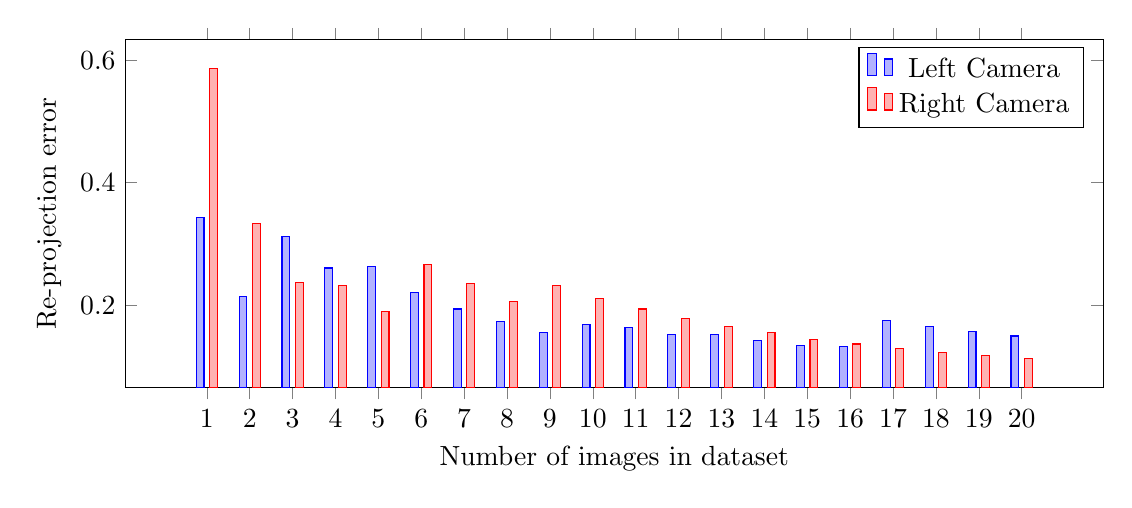
\begin{tikzpicture}
 
    \begin{axis} [ybar,
        height=6cm,
        width=14cm,
        bar width=0.1cm, 
        xlabel={Number of images in dataset}, 
        ylabel={Re-projection error},
        xtick={1,2,3,4,5,6,7,8,9,10,11,12,13,14,15,16,17,18,19,20}
        ]
     
    \addplot coordinates {(1, 0.343) (2, 0.214) (3, 0.312) (4, 0.261) (5, 0.263) (6, 0.221) (7, 0.194) (8, 0.173) (9, 0.156) (10, 0.169) (11, 0.164) (12, 0.153) (13, 0.153) (14, 0.143) (15, 0.135) (16, 0.133) (17, 0.175) (18, 0.166) (19, 0.158) (20, 0.150) };
    \addplot coordinates {(1, 0.586) (2, 0.333) (3, 0.237) (4, 0.232) (5, 0.190) (6, 0.266) (7, 0.235) (8, 0.207) (9, 0.232) (10, 0.211) (11, 0.194) (12, 0.178) (13, 0.166) (14, 0.155) (15, 0.145) (16, 0.137) (17, 0.129) (18, 0.123) (19, 0.118) (20, 0.113) };
     
    \legend {Left Camera, Right Camera};
     
    \end{axis}
 
    \end{tikzpicture}
    \caption{Analysing how the size of the dataset affects calibration quality}
    \label{fig:camera calibration}
\end{figure}

\section{Ball Detection}

After a calibrated image is retrieved, a decision must be made as to how to process the image in order to locate the position of the ball - or how to tackle the problem of object detection. A neural approach such as a convolutional neural network can produce very impressive results, however due to their computational complexity they are not appropriate for this project. This means that a non-neural approach must be taken. 

A common solution is to use a sliding window, classifying each area of the image to find the position of the ball. However this method requires hundreds or even thousands of areas to be classified meaning that a feature vector must be generated and evaluated for every area, which is a very computationally expensive process. This is not feasible for this project so a more efficient solution is required.

The method chosen can be broken down into two steps; an feature extraction algorithm to produce a list of potential ball candidates and a set of filters to remove false positives from this list.

\begin{figure}[H]
    \centering
    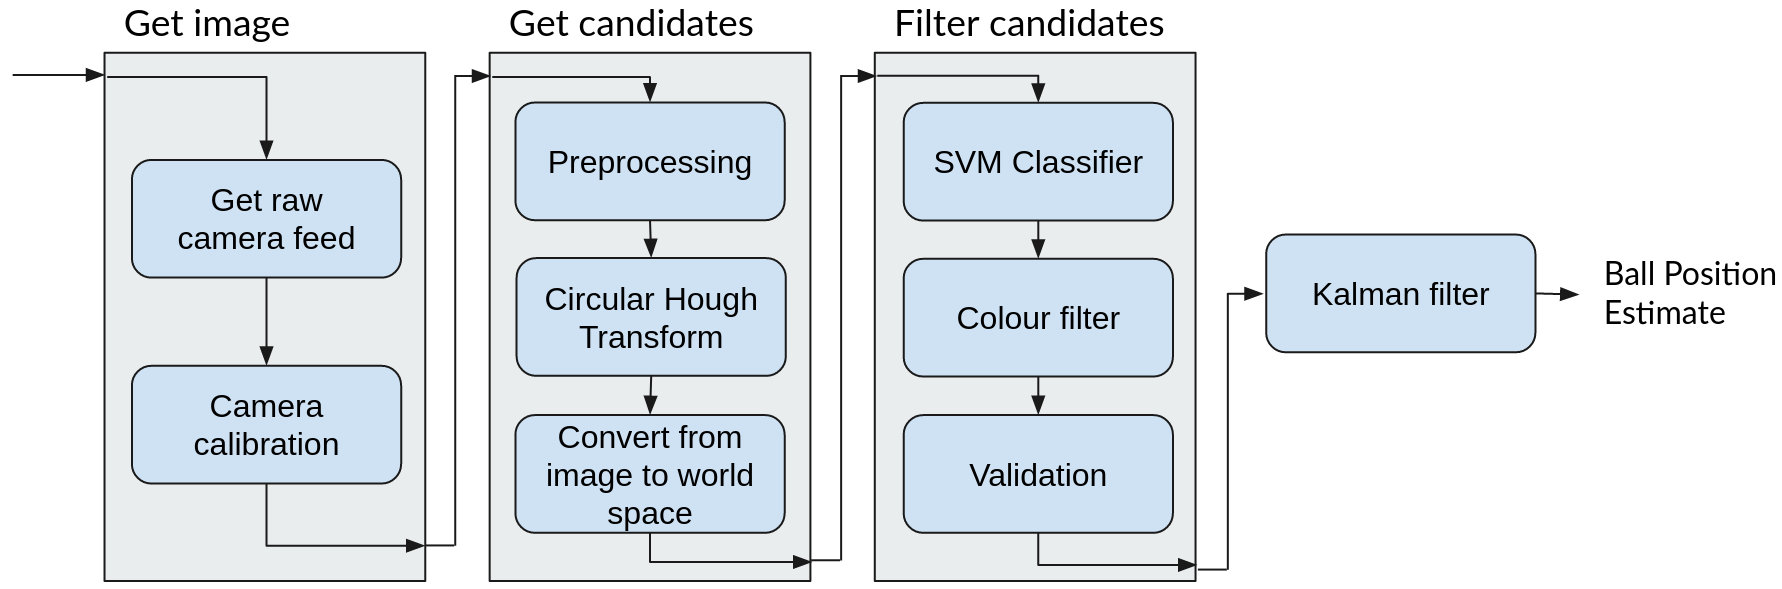
\includegraphics[width=16cm]{images/position-design.png}
    \caption{Flow diagram for ball position design}
    \label{fig:position design}
\end{figure}

\subsection{Get Candidates}

\subsubsection{Circular Hough Transform}
\label{section: Hough design}

The circular Hough transform is used to generate a list of ball candidates from the image. This algorithm was chosen for this task as it can produce reliable results very efficiently compared to alternative feature extraction techniques such as blob detection. However this efficiency comes at a cost of needing a well segmented mask, meaning that circular shapes have to be detected by colour. As well as decreasing robustness to changes in lighting and ball pattern, this requires that the ball is a different colour to the floor and walls of the pitch. 

\subsubsection{Preprocessing}

The raw camera feed must be converted to a mask so that the circular Hough transform can more reliably detect the ball. This mask is produced by colour segmentation. Any pixels that match the colours of the ball, or are within a range of these colours, are included in the mask while other pixels are discarded, resulting in a binary image. For this task the image is converted to the HSV colour space, which is preferred to RGB as it is easier to define ranges for the colour thresholding. This mask is then cleaned up using a Gaussian blur as well as erode and dilate operations to reduce noise.

\subsubsection{Image to World Space Conversion}

For this conversion there are three relevant spaces: image space, head space and world space. A position in image space is a 2-dimensional coordinate representing a pixel in the image, with the origin in the top left corner. A position in head space is a 3-dimensional coordinate representing the position of a point, relative to the transformation of MiRo's head. The origin of this space is equal to the position of the head. A position in world space is a 3-dimensional coordinate representing a point in the world, completely unrelated to the MiRo. This means that any position in image or head space is specific to one agent, whereas a position in world space can be understood by any agent.

To convert from image space to world space, the pixel coordinate is converted to a position in head space using an estimated distance of the ball. This is then converted to world space using information about the current robot kinematics and position in the world. 

\begin{figure}[ht]
    \begin{subfigure}[b]{0.4\textwidth}
        \centering
        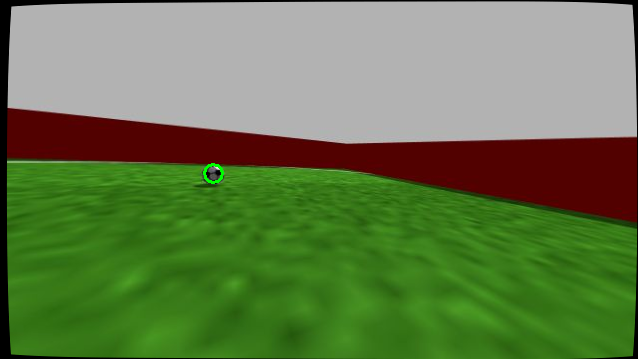
\includegraphics[width=6cm]{images/imagespace.png}
    \end{subfigure}
    %
    \begin{subfigure}[b]{0.4\textwidth}
        \centering
        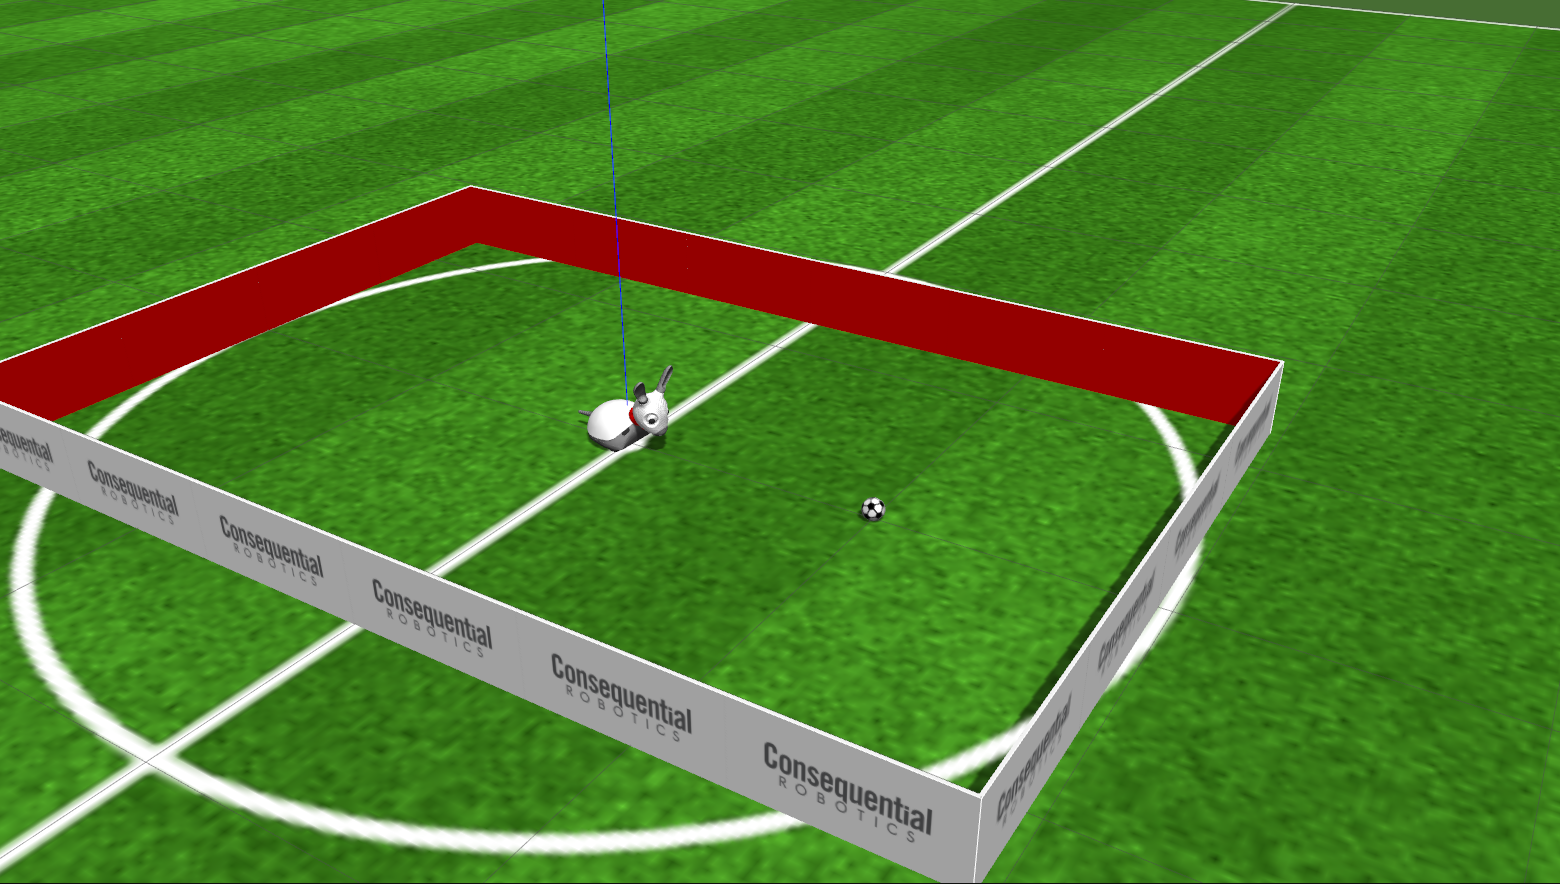
\includegraphics[width=6cm]{images/worldspace.png}
    \end{subfigure}
\centering

In this scenario, the ball is at $\begin{bmatrix}214 & 174 \end{bmatrix}$ in image space and $\begin{bmatrix}-1 & 0 & 0.04 \end{bmatrix}$ in world space. Therefore the position in head space is $\begin{bmatrix}1 & 0 & -0.2 \end{bmatrix}$. The $x$ value is positive as the MiRo is facing the ball and the $z$ value is negative as the ball is below the height of the head.
\caption{Illustrating image space and world space}
\end{figure}

\subsection{Filter Candidates}

\subsubsection{SVM Classifier}
\label{section: svm-hog}

The primary filter is a classifier that evaluates whether an area of the image is a ball. The classifier uses the histogram of oriented gradients (HOG) feature descriptor to summarise the shape information of the area. HOG is preferred to other feature descriptors such as SURF or SIFT as it is computationally efficient enough to run in real time and proven in object detection problems. A support-vector machine (SVM) is the favoured classifier as it is also well documented in this problem, especially in combination with the HOG feature, and was found to be more efficient than other options such as a decision tree classifier. Analysis of the performance of classifiers can be found in \ref{section: svm-implement}.

\subsubsection{Colour Filter}
\label{section: colour filter design}

The second filter takes advantage of the colour information of the image, using K-means clustering to extract the most common colours of the image. If these most common colours do not match that of the ball then the candidate can be rejected. The purpose of this filter is to reject candidates that have been missed by the classifier due to having a similar shape to the ball and to reject candidates that might contain the ball as well as a larger area surrounding it which could lead to inaccuracies in position estimation.

\subsubsection{Validation}

Some validation is performed on the candidates using their world positions. The first is to reject any candidates that are outside the borders of the pitch, although there is some leeway to allow for small errors in position when the ball is at the edge of the pitch. Another validation is to check that the candidate is not too far from previous estimates. This uses a normal distribution on the last 10 positions (approximately 1 second) as well as 5 future predictions at intervals of $1/10$ seconds to account for the expected movement of the ball. Any positions that are not within 3 standard deviations of this distribution are rejected. The last validation is to limit there to only be one candidate for each image. The best candidate is chosen by comparing the confidence value of classifier's evaluation.
 
 \subsection{Kalman Filter}
 
These final ball positions are then fed into a Kalman filter which uses a combination of a prediction model and perceived positions to output a best estimate of the current position of the ball in world space. The Kalman filter is favoured over other fusion techniques due to having good performance on kinematic problems like this one and its much greater computational efficiency than options such as Monte Carlo Localisation. 

The filter uses the state vector

\[\hat{x}_{k|k} = \begin{bmatrix}position_x \\ position_y \\ velocity_x \\ velocity_y\end{bmatrix}\]

\noindent and the transition function

\[F_k = \begin{bmatrix} 1 & 0 & \Delta t & 0 \\ 0 & 1 & 0 & \Delta t \\ 0 & 0 & 1 & 0 \\ 0 & 0 & 0 & 1\end{bmatrix}\]

This assumes that the ball velocity is constant between updates, which is an acceptable assumption as there is a short time between updates (100ms) and noise in the data makes calculating any change in the velocity unreliable. 


\section{Ball Velocity}

\begin{figure}[H]
    \centering
    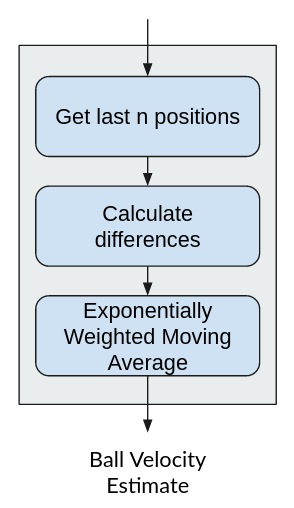
\includegraphics[width=4cm]{images/velocity-design.png}
    \caption{Flow diagram for ball velocity design}
    \label{fig:velocity design}
\end{figure}

Ball velocity is estimated using a list of the most recent ball position estimates. The difference between each adjacent position is calculated and an exponentially weighted moving average (EWMA) is performed on the differences to give an estimate for velocity. EWMA is chosen so that more recent values have a greater contribution to the average, meaning that the system can react to changes in velocity more quickly.

\section{Trajectory Prediction}

\begin{figure}[H]
    \centering
    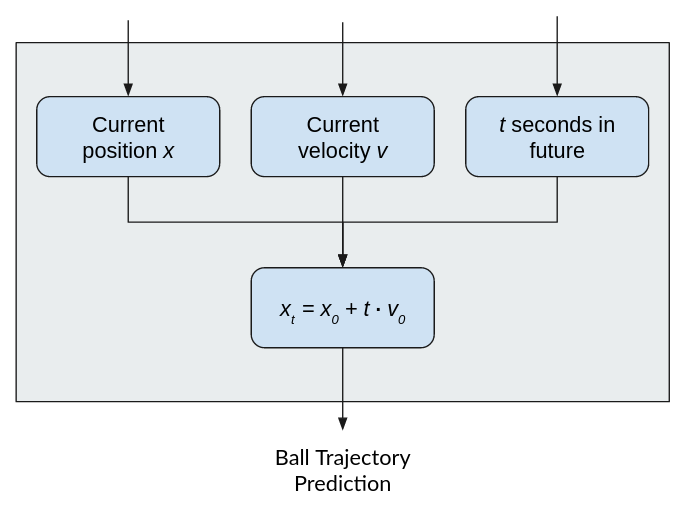
\includegraphics[width=9cm]{images/trajectory-design.png}
    \caption{Flow diagram for ball trajectory design}
    \label{fig:trajectory design}
\end{figure}

The trajectory of the ball is estimated using the kinematic equation:
\[ x_t = x_0 + t \cdot v_0 \]
Where $x$ is the future position, $x_0$ is the current position, $v_0$ is the current velocity and $t$ is the time in the future to estimate the position for. This method is used due to its simplicity, however a more advanced technique could provide more accurate results. 

\chapter{Implementation and Testing}
\label{chapter: 5}

This chapter describes how the biggest challenges in the project were overcome, giving detail on the development process and exact parameters that are used in the algorithms. 

\section{Notable Algorithms}

\subsection{Circular Hough Transform}

Ball candidates are obtained from the image using the OpenCV implementation of the circular Hough transform. The minimum ball radius is set to 4 pixels, as candidates smaller than this do not contain enough information to confidently decide whether the candidate is a true positive. This values limits the maximum distance that the ball can be detected from though the trade-off is justified by greatly reducing the number of false positives. The maximum ball radius is set to 40 as it is not possible for the ball to be any bigger than this in the image. The sensitivity parameter causes more or fewer circles to be detected in the image and represents a trade-off between decreasing the likelihood that the ball is missed and a longer computation time of analysing and rejecting more false positives. The value for this was decided empirically to be 10. 

\begin{figure}[H]
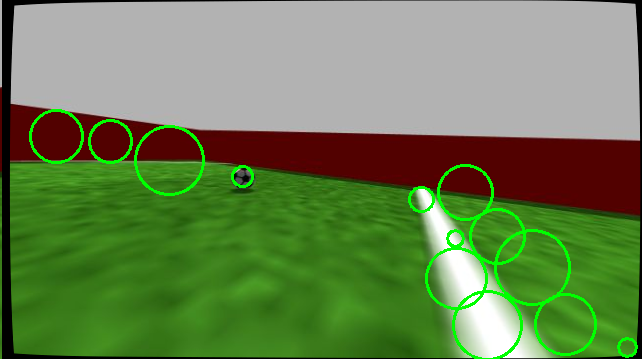
\includegraphics[width=7cm]{images/hough.png}
\centering
\caption{An example output of the circular Hough transform}
\end{figure}

\subsection{SVM Classifier}
\label{section: svm-implement}

The classifier uses the histogram of oriented gradients feature vector to decide whether a ball candidate should be rejected. The HOG descriptor uses the scikit-image implementation and uses a cell size of 8x8 pixels and a block size of 2x2 cells. All images are resized to 32x32 pixels as the SVM requires that every input vector must be the same size. A size of 32 pixels was chosen as ball candidate image usually smaller than this size meaning that no data is lost by resizing, while still being small enough to be able to compute quickly. These factors result in the feature vector having 288 dimensions.

Two datasets were collected for training the classifier; one in simulation and one on a real ball. Each dataset contains approximately 2000 negative samples and 200 positive samples. The positive samples are augmented by horizontal mirroring and rotations of -20\degree, -10\degree, 10\degree, 20\degree to increased the number of samples 10 times. Therefore there are also effectively 2000 positive samples, and the classifier is trained on approximately 4000 images. The datasets were collected by storing images of ball candidates that the system detected during the running of a basic ball chasing script. Each image was then manually labelled. 

Figure \ref{fig:comparing classifiers} shows the results of the comparison of various classifiers: k-nearest neighbours (k=5), k-nearest neighbours (k=15), linear SVM, SVM using the radial basis function (RBF) kernel, random forest and AdaBoost. Of these the SVM using the RBF kernel had the best results with a precision of 99.2\% and a recall of 96.1\% while having the second best classify time, only marginally slower than the linear SVM. Therefore the SVM with RBF kernel is the classifier used in the final implementation.

\begin{figure}[H]
    \centering
    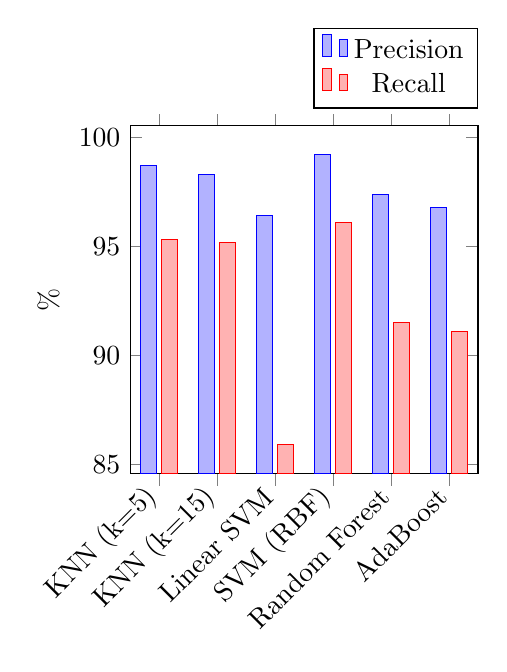
\begin{tikzpicture}
        \begin{axis} [ybar,
            height=6cm,
            width=6cm,
            bar width=0.2cm, 
            xlabel={}, 
            ylabel={\%},
            xtick={0,1,2,3,4,5},
            xticklabels={KNN (k=5), KNN (k=15), Linear SVM, SVM (RBF), Random Forest, AdaBoost},
            % xticklabels={Precision, Recall},
            xlabel style={yshift=-1cm},
            x tick label style={
                rotate=45,
                anchor=east,
            },
            legend style={
                anchor=south east,
                at={(1,1.05)}
                }
            ]
        \addplot coordinates {(1, 98.3) (0, 98.7) (2, 96.4) (3, 99.2) (4, 97.4) (5, 96.8)};
        \addplot coordinates {(1, 95.2) (0, 95.3) (2, 85.9) (3, 96.1) (4, 91.5) (5, 91.1)};
        
        % \addplot coordinates {(0, 98.3) (1, 95.2)};
        % \addplot coordinates {(0, 96.4) (1, 85.9)};
        % \addplot coordinates {(0, 99.2) (1, 96.1)};
        % \addplot coordinates {(0, 97.7) (1, 90.0)};
        % \addplot coordinates {(0, 96.8) (1, 91.1)};
        
        \legend {Precision, Recall};
        \end{axis}
    \end{tikzpicture}
    \hfill
    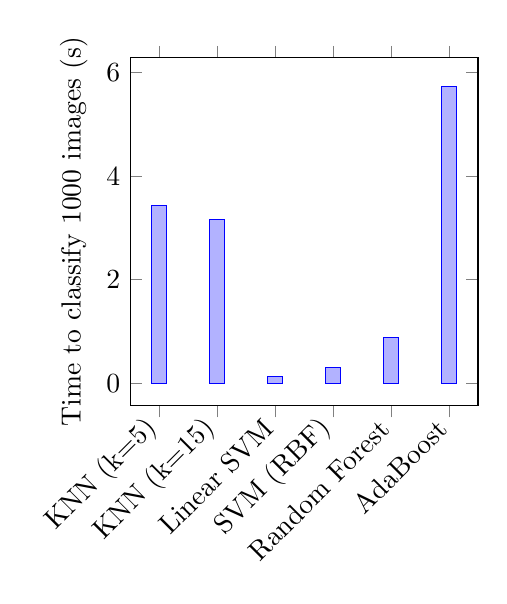
\begin{tikzpicture}
        \begin{axis} [ybar,
            height=6cm,
            width=6cm,
            bar width=0.2cm, 
            xlabel={}, 
            ylabel={Time to classify 1000 images (s)},
            xtick={0,1,2,3,4,5},
            xticklabels={KNN (k=5), KNN (k=15), Linear SVM, SVM (RBF), Random Forest, AdaBoost},
            xlabel style={yshift=-1cm},
            x tick label style={
                rotate=45,
                anchor=east,
            }
            ]
        \addplot coordinates {(1,3.163) (0, 3.43) (2,0.125) (3,0.299) (4,0.875) (5,5.729)};
        \end{axis}
    \end{tikzpicture}
    
    \caption{Comparing the performance of classifiers}
    \label{fig:comparing classifiers}
\end{figure}

\subsection{Image to World Space Conversion}
\label{section: image to world}

The MiRo Development Kit provides functions to convert a coordinate in image space and a range to a coordinate in world space. A view line is taken from the camera through the image space position, and a position can be found in head space by taking the position on the line corresponding to the range. The position in head space is then mapped into world space using the kinematic data of the MiRo. 

The range can be estimated by various methods. The first is to use a function mapping the radius of the ball in the image to a range, however this proved to be very noisy even when the ball is static. Another option is to obtain depth information from the image. Stereo depth is the obvious choice as the MiRo has stereo vision, however this limits the information to only the region shared by both cameras, and is time-consuming to tune to a reasonable accuracy. 

Instead of using the range to find the position on the view line, the final system uses the assumption that the ball is on the floor. This means that the z coordinate of the world position is already known to be at the center of the ball, or its radius so final coordinate can be calculated by finding the point at which the view line intercepts this height. 

This method results in more precise estimations, however there is a systematic error that can greatly decrease accuracy caused by imperfections in the camera calibration. The error can be corrected by applying offsets the azimuth and altitude of the view line according to the image space coordinates. 
The error in the azimuth correlates is fitted to a sine wave in the image x position and the altitude error is fitted to a polynomial regression in the image y position. As these corrections are specific to a camera calibration, they must be calculated independently for each MiRo. 

\subsubsection{Horizontal Coordinate System}

The horizontal coordinates system is a coordinate system that can be used to describe a 3-dimensional vector using 2 values. These values are the azimuth, which describes a rotation about the Z-axis or zenith and the altitude, which describes the rotation across the XY-plane.

\begin{figure}[H]
    \centering
    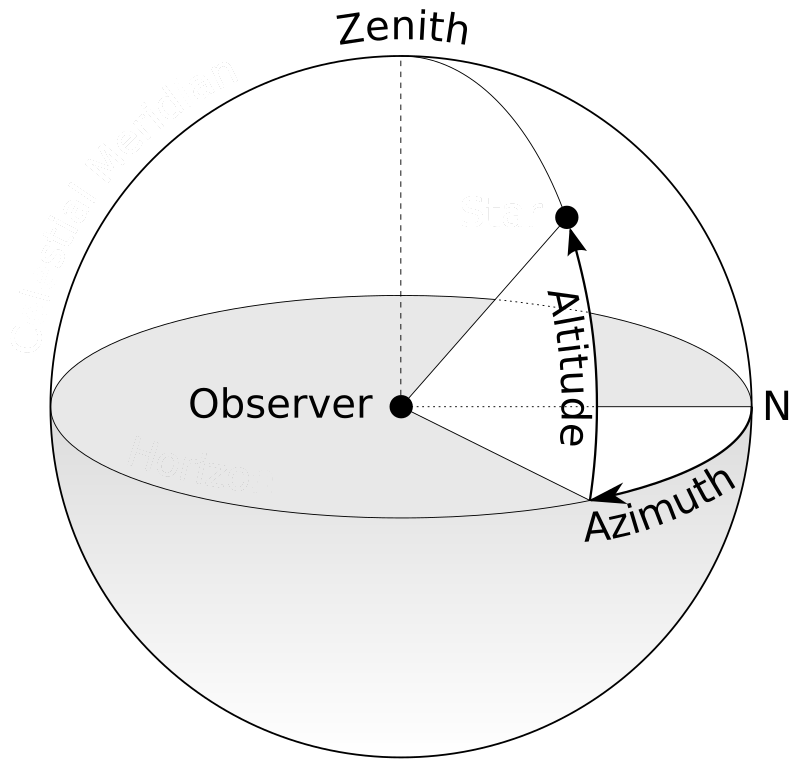
\includegraphics[width=7cm]{images/azal.png}
    \caption{Illustrating horizontal space coordinates}
    \label{fig:horizontal coordinates}
    Source: \url{https://en.wikipedia.org/wiki/Horizontal_coordinate_system} (edited)
\end{figure}

\chapter{Results and Discussion}
\label{chapter: 6}

This chapter outlines how results are obtained from the system and uses these results to discuss how successful the project was. Ideas for future work related to the project are included as well. 

\section{Results}

In order to evaluate the performance of the system after it has finished, some data is recorded. On every tick a new record is saved, containing data points for useful information such as estimated ball position and velocity. As well as this, data is stored for each accepted ball candidate including the candidate's image and world position. The tests described in the following sections will be performed using this data. 

The system will be run through a set of six scenarios to test the performance in various situations, shown in figure \ref{fig: scenarios}. The first three tests contain only the MiRo and the ball, with the ball moving across the MiRo, away from it and towards it respectively. The last three tests use the same ball motion, but include another MiRo to interfere with the perception system. In scenarios 4 and 6 the ball passes in front of the other MiRo, and passes behind in scenario 5, obscured vision for a period of time. The tests will be run in simulation as this allows the real position of the ball to easily be recorded, and the tests can be easily repeated. To get a robust average of results the test will be repeated 20 times. 

\begin{figure}[H]
    \begin{tikzpicture} 
    \begin{axis} [
        ymin=-1.3,
        ymax=1.3,
        xmin=-1.95,
        xmax=1.95,
        xlabel=Scenario 1
    ]
    \addplot [only marks] table {
0 0
};
\addplot [only marks, mark=o] table {
1 -1
1 1.15
};
\draw[->] (axis cs:1,-1) -- (axis cs:1,1.15);
    \end{axis} 
    \end{tikzpicture}
%
\begin{tikzpicture} 
    \begin{axis} [
        ymin=-1.3,
        ymax=1.3,
        xmin=-1.95,
        xmax=1.95,
        xlabel=Scenario 2
    ]
    \addplot [only marks] table {
0 0
};
\addplot [only marks, mark=o] table {
0 1
1.5 0.35
};
\draw[->] (axis cs:0,1) -- (axis cs:1.5,0.35);
    \end{axis} 
\end{tikzpicture}

\begin{tikzpicture} 
    \begin{axis} [
        ymin=-1.3,
        ymax=1.3,
        xmin=-1.95,
        xmax=1.95,
        xlabel=Scenario 3
    ]
    \addplot [only marks] table {
0 0
};
\addplot [only marks, mark=o] table {
1.5 0.5
-0.3 -0.725
};
\draw[->] (axis cs:1.5,0.5) -- (axis cs:-0.3,-0.725);
    \end{axis} 
\end{tikzpicture}
%
    \begin{tikzpicture} 
    \begin{axis} [
        ymin=-1.3,
        ymax=1.3,
        xmin=-1.95,
        xmax=1.95,
        xlabel=Scenario 4
    ]
    \addplot [only marks] table {
0 0
};
\addplot [only marks, mark=o] table {
1 -1
1 1.15
};
\addplot [only marks, mark=triangle] table {
1.5 0.2
};
\draw[->] (axis cs:1,-1) -- (axis cs:1,1.15);
    \end{axis} 
    \end{tikzpicture}

\begin{tikzpicture} 
    \begin{axis} [
        ymin=-1.3,
        ymax=1.3,
        xmin=-1.95,
        xmax=1.95,
        xlabel=Scenario 5
    ]
    \addplot [only marks] table {
0 0
};
\addplot [only marks, mark=o] table {
0 1
1.5 0.35
};
\addplot [only marks, mark=triangle] table {
0.5 0.5
};
\draw[->] (axis cs:0,1) -- (axis cs:1.5,0.35);
    \end{axis} 
\end{tikzpicture}
%
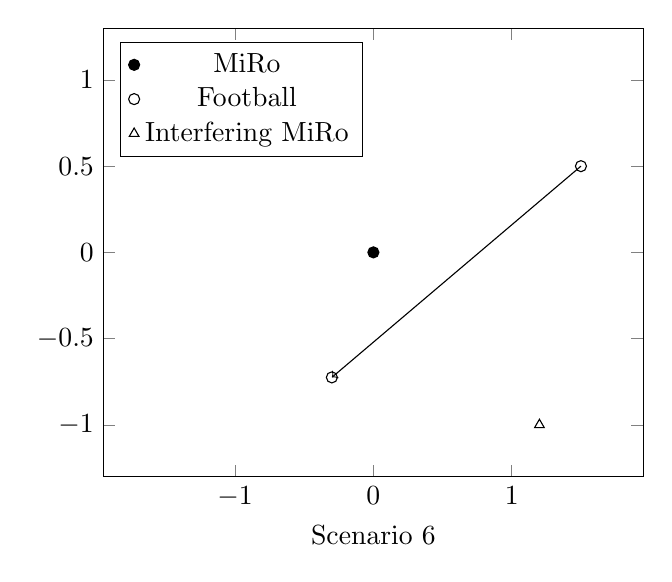
\begin{tikzpicture} 
    \begin{axis} [
        ymin=-1.3,
        ymax=1.3,
        xmin=-1.95,
        xmax=1.95,
        xlabel=Scenario 6,
        legend style={at={(0.03,0.97)},anchor=north west}
    ]
    \addplot [only marks] table {
0 0
};
\addlegendentry{MiRo}
\addplot [only marks, mark=o] table {
1.5 0.5
-0.3 -0.725
};
\addlegendentry{Football}
\addplot [only marks, mark=triangle] table {
1.2 -1
};
\addlegendentry{Interfering MiRo}
\draw[->] (axis cs:1.5,0.5) -- (axis cs:-0.3,-0.725); 
    \end{axis} 
\end{tikzpicture}
\caption{Scenarios used to evaluate the system}
\label{fig: scenarios}
\end{figure}

\subsection{Ball Position}

\subsubsection{Relative Error}

The primary metric for the accuracy of the ball position estimation uses relative error. This is preferred over absolute error as it is more lenient when the ball is far away, and more strict when the ball is close. The relative error is used to calculate an overall score as a percentage, where 100\% is perfect accuracy and 0\% is infinitely inaccurate. 

\[ \text{Absolute error: } \epsilon =  |v - v_{estimate}|\]
\[ \text{Relative error: } \eta =  |1 - \frac{v_{estimate}}{v}|\]
\[ \text{Overall score: } s = \frac{1}{e^{\eta}} \]
Where $v$ is a value and $v_{estimate}$ is the estimated value.

\begin{figure}[H]
    \centering
    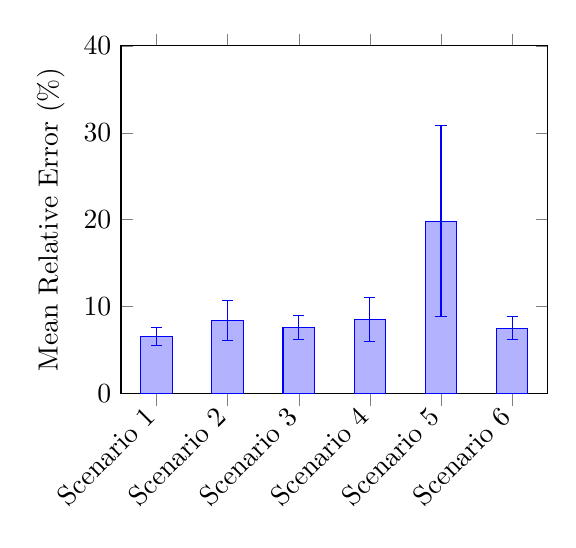
\begin{tikzpicture}
 
    \begin{axis} [ybar,
        height=6cm,
        width=7cm,
        bar width=0.4cm, 
        xlabel={}, 
        ylabel={Mean Relative Error (\%)},
        xtick={1,2,3,4,5,6},
        ymin=0,
        ymax=40,
        xticklabels={Scenario 1,Scenario 2,Scenario 3,Scenario 4,Scenario 5,Scenario 6},
        xlabel style={yshift=-1cm},
            x tick label style={
                rotate=45,
                anchor=east,
            }
        ]
     
     \addplot+ [
            error bars/.cd,
                y dir=both,
                y explicit relative,
        ] coordinates {
            (1,6.585) +- (0,0.04095*4)
            (2,8.413) +- (0,0.06813*4)
            (3,7.629) +- (0,0.04601*4)
            (4,8.514) +- (0,0.07422*4)
            (5,19.840) +- (0,0.13862*4)
            (6,7.536) +- (0,0.04379*4)
        };
     
    \end{axis}
 
    \end{tikzpicture}
    \hfill
    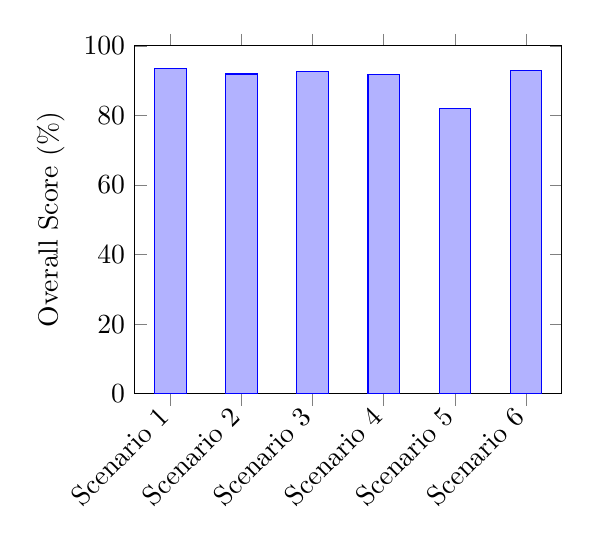
\begin{tikzpicture}
 
    \begin{axis} [ybar,
        height=6cm,
        width=7cm,
        bar width=0.4cm, 
        xlabel={}, 
        ylabel={Overall Score (\%)},
        xtick={1,2,3,4,5,6},
        ymin=0,
        ymax=100,
        xticklabels={Scenario 1,Scenario 2,Scenario 3,Scenario 4,Scenario 5,Scenario 6},
        xlabel style={yshift=-1cm},
            x tick label style={
                rotate=45,
                anchor=east,
            }
        ]
     
     \addplot coordinates {(1,93.6) (2,91.9) (3,92.7) (4,91.8) (5,82.0) (6,92.8)};
     
    \end{axis}
 
    \end{tikzpicture}
    \caption{Mean relative error for each scenario}
    \label{fig:position error}
\end{figure}


Figure \ref{fig:position error} shows the results of this experiment. The system has overall good performance with 5/6 of the scenarios having a relative error of less than 10\%. All scenarios without another MiRo on the pitch showed good accuracy, as well as the scenarios where the ball passed in front of another MiRo. However when the ball passed behind a MiRo and was obscured in scenario 5, the average relative error increased to around 20\%, and there was a much greater variance in accuracy. 

The average score of the system over all six scenarios was 90.8\%, which is accurate enough to be reasonably used in a game of robot football.
 
\subsubsection{Direction and Range Error}

In order to better understand what is causing the error in position, the error can be split into two metrics: direction error and distance error. The direction error represents the difference between the estimated ball position and the MiRo, and the real ball position and the MiRo. The absolute error is used as a higher angle has no impact on the expected accuracy. The distance error represents the error in the estimated distance to the ball compared to the real distance to the ball. 

\begin{figure}[H]
    \centering
    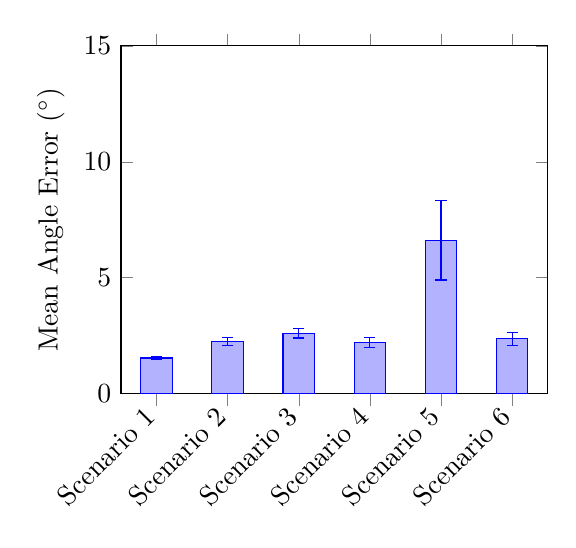
\begin{tikzpicture}
 
    \begin{axis} [ybar,
        height=6cm,
        width=7cm,
        bar width=0.4cm, 
        xlabel={}, 
        ylabel={Mean Angle Error (\degree)},
        xtick={1,2,3,4,5,6},
        ymin=0,
        ymax=15,
        xticklabels={Scenario 1,Scenario 2,Scenario 3,Scenario 4,Scenario 5,Scenario 6},
        xlabel style={yshift=-1cm},
            x tick label style={
                rotate=45,
                anchor=east,
            }
        ]
        
     \addplot+ [
            error bars/.cd,
                y dir=both,
                y explicit relative,
        ] coordinates {
            (1,1.541) +- (0,0.01266*4)
            (2,2.247) +- (0,0.02021*4)
            (3,2.612) +- (0,0.02022*4)
            (4,2.204) +- (0,0.02376*4)
            (5,6.622) +- (0,0.06482*4)
            (6,2.364) +- (0,0.02935*4)
        };
     
    \end{axis}
 
    \end{tikzpicture}
    \hfill
    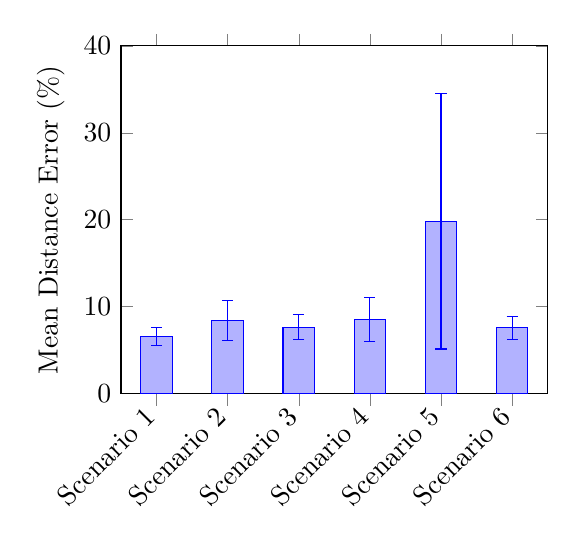
\begin{tikzpicture}
 
    \begin{axis} [ybar,
        height=6cm,
        width=7cm,
        bar width=0.4cm, 
        xlabel={}, 
        ylabel={Mean Distance Error (\%)},
        xtick={1,2,3,4,5,6},
        ymin=0,
        ymax=40,
        xticklabels={Scenario 1,Scenario 2,Scenario 3,Scenario 4,Scenario 5,Scenario 6},
        xlabel style={yshift=-1cm},
            x tick label style={
                rotate=45,
                anchor=east,
            }
        ]
     
     \addplot+ [
            error bars/.cd,
                y dir=both,
                y explicit relative,
        ] coordinates {
            (1,6.577) +- (0,0.04081*4)
            (2,8.409) +- (0,0.06801*4)
            (3,7.649) +- (0,0.04613*4)
            (4,8.514) +- (0,0.07409*4)
            (5,19.848) +- (0,0.1853*4)
            (6,7.564) +- (0,0.04411*4)
        };
     
    \end{axis}
 
    \end{tikzpicture}
    \caption{Mean direction error and relative distance error}
    \label{fig:direction distance error}
\end{figure}

At first glance these results show the same outcome of the previous - that the accuracy is good aside from scenario 5. However looking at the results as a whole, it is clear that the direction error is overall very low with most scenarios having an average error below 3\degree and a small standard deviation, which has a small impact on the relative error of the position. However the average distance error is overall greater and is more often the reason for inaccurate estimations. 

\subsection{Ball Velocity}

To measure the accuracy of the ball velocity estimation, a similar metric to the relative error in the previous section will be used. In order to avoid undefined values when the velocity is zero, a small offset, $a$, will be added to the real velocity. 

\[ \text{Relative error (with offset): } \eta_a =  |1 - \frac{v_{estimate}}{v + a}|\]

\begin{figure}[H]
    \centering
    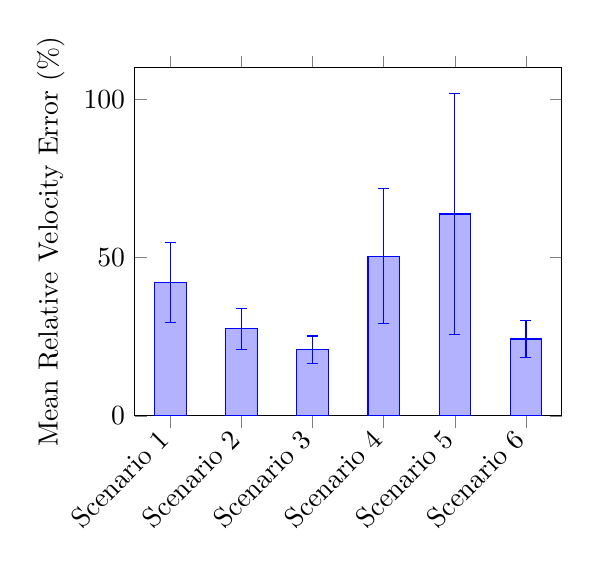
\begin{tikzpicture}
 
    \begin{axis} [ybar,
        height=6cm,
        width=7cm,
        bar width=0.4cm, 
        xlabel={}, 
        ylabel={Mean Relative Velocity Error (\%)},
        xtick={1,2,3,4,5,6},
        ymin=0,
        ymax=110,
        xticklabels={Scenario 1,Scenario 2,Scenario 3,Scenario 4,Scenario 5,Scenario 6},
        xlabel style={yshift=-1cm},
            x tick label style={
                rotate=45,
                anchor=east,
            }
        ]
     
     \addplot+ [
            error bars/.cd,
                y dir=both,
                y explicit relative,
        ] coordinates {
            (1,42.160) +- (0,29.768*0.01)
            (2,27.524) +- (0,23.697*0.01)
            (3,20.945) +- (0,20.499*0.01)
            (4,50.469) +- (0,42.429*0.01)
            (5,63.813) +- (0,59.552*0.01)
            (6,24.277) +- (0,23.994*0.01)
        };
     
    \end{axis}
 
    \end{tikzpicture}
    \caption{Mean relative velocity error for each scenario, $a=1$}
    \label{fig:velocity error}
\end{figure}

These results are interesting as they do not match the the results for the ball position. Scenarios 1 and 4 are considerably less accurate than 2,3 and 6 despite all having similar scores in figure \ref{fig:position error}. One reason for this could be shown in figure \ref{figure: x vs y}, which shows every position estimation that the system made during the scenarios. The estimations for scenarios 2,3 and 6 are all reasonably straight lines, as expected, however the data points for scenarios 1 and 4 form a slight curve, bowing outwards in the centre. This curve seems to be caused by the ball moving both towards and away from the MiRo during these scenarios, showing inaccuracy in the estimation of the distance to the ball. 

\begin{figure}[H]
    \centering
    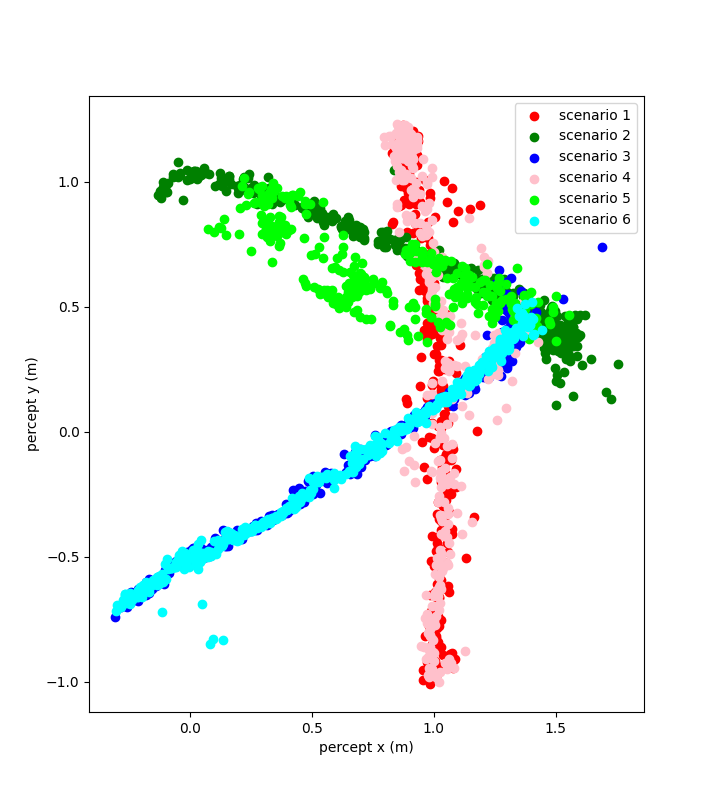
\includegraphics[width=15cm]{images/x_y.png}
    \caption{Plotting every ball position estimation}
    \label{figure: x vs y}
\end{figure}

\subsection{Ball Trajectory}
\label{section: trajectory results}

In order to measure the accuracy of the ball trajectory prediction, the relative error between the real ball position $t$ seconds in the future and the predicted position at that time is calculated. This means that the last $t$ seconds of each scenario will not be included in the measurement. As the data is collected from the simulation, which does not simulate friction for the ball, the results are expected to be better than in a more realistic situation.

\begin{figure}[H]
    \centering
    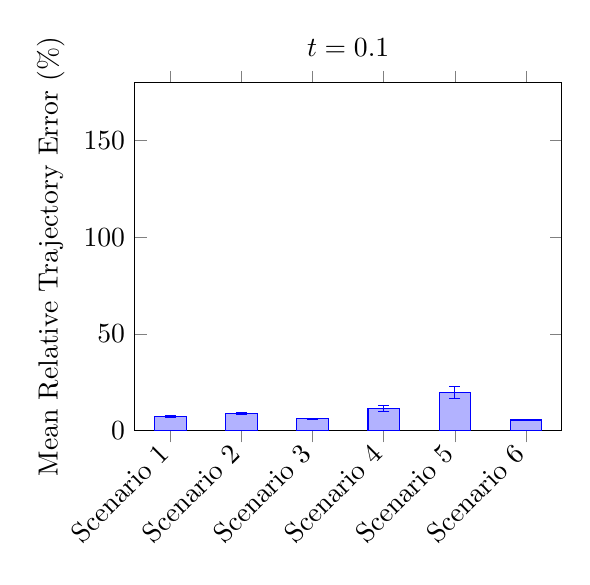
\begin{tikzpicture}
 
    \begin{axis} [ybar,
        title={$t=0.1$},
        height=6cm,
        width=7cm,
        bar width=0.4cm, 
        xlabel={}, 
        ylabel={Mean Relative Trajectory Error (\%)},
        xtick={1,2,3,4,5,6},
        ymin=0,
        ymax=180,
        xticklabels={Scenario 1,Scenario 2,Scenario 3,Scenario 4,Scenario 5,Scenario 6},
        xlabel style={yshift=-1cm},
            x tick label style={
                rotate=45,
                anchor=east,
            }
        ]
     
     \addplot+ [
            error bars/.cd,
                y dir=both,
                y explicit relative,
        ] coordinates {
            (1,7.252) +- (0,5.654*0.01)
            (2,8.828) +- (0,5.940*0.01)
            (3,6.085) +- (0,4.588*0.01)
            (4,11.304) +- (0,13.462*0.01)
            (5,19.822) +- (0,15.417*0.01)
            (6,5.450) +- (0,4.278*0.01)
        };
     
    \end{axis}
 
    \end{tikzpicture}
    \hfill
    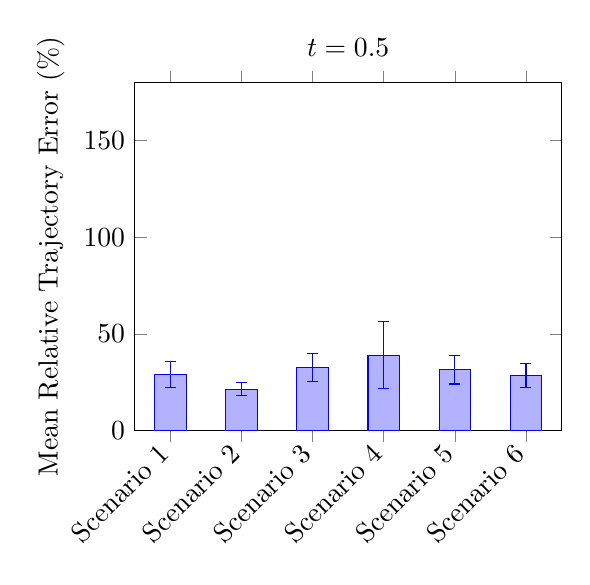
\begin{tikzpicture}
 
    \begin{axis} [ybar,
        title={$t=0.5$},
        height=6cm,
        width=7cm,
        bar width=0.4cm, 
        xlabel={}, 
        ylabel={Mean Relative Trajectory Error (\%)},
        xtick={1,2,3,4,5,6},
        ymin=0,
        ymax=180,
        xticklabels={Scenario 1,Scenario 2,Scenario 3,Scenario 4,Scenario 5,Scenario 6},
        xlabel style={yshift=-1cm},
            x tick label style={
                rotate=45,
                anchor=east,
            }
        ]
     
     \addplot+ [
            error bars/.cd,
                y dir=both,
                y explicit relative,
        ] coordinates {
            (1,29.133) +- (0,22.886*0.01)
            (2,21.425) +- (0,16.319*0.01)
            (3,32.503) +- (0,22.472*0.01)
            (4,38.977) +- (0,44.633*0.01)
            (5,31.541) +- (0,23.690*0.01)
            (6,28.495) +- (0,21.457*0.01)
        };
     
    \end{axis}
 
    \end{tikzpicture}
    
    
    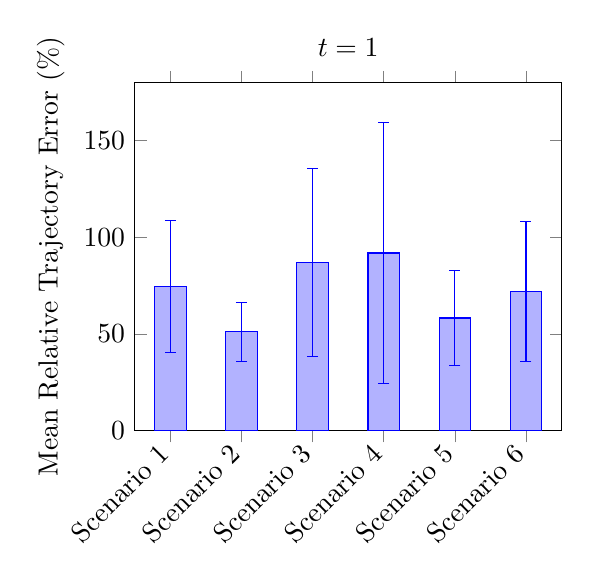
\begin{tikzpicture}
 
    \begin{axis} [ybar,
        title={$t=1$},
        height=6cm,
        width=7cm,
        bar width=0.4cm, 
        xlabel={}, 
        ylabel={Mean Relative Trajectory Error (\%)},
        xtick={1,2,3,4,5,6},
        ymin=0,
        ymax=180,
        xticklabels={Scenario 1,Scenario 2,Scenario 3,Scenario 4,Scenario 5,Scenario 6},
        xlabel style={yshift=-1cm},
            x tick label style={
                rotate=45,
                anchor=east,
            }
        ]
     
     \addplot+ [
            error bars/.cd,
                y dir=both,
                y explicit relative,
        ] coordinates {
            (1,74.725) +- (0,45.689*0.01)
            (2,51.012) +- (0,30.272*0.01)
            (3,87.051) +- (0,55.774*0.01)
            (4,91.819) +- (0,73.479*0.01)
            (5,58.210) +- (0,42.155*0.01)
            (6,71.909) +- (0,50.203*0.01)
        };
     
    \end{axis}
 
    \end{tikzpicture}
    \caption{Mean relative trajectory error for each scenario, $t$ seconds in the future}
    \label{fig:trajectory error}
\end{figure}

When $t = 0.1$, or when the prediction is for the next system iteration, there is already considerable error in the trajectory prediction, especially in scenario 5 which has seen poor results in the previous tests. This inaccuracy grows as $t$ increases, reaching over 100\% error at times when $t$ = 1. These results are not accurate enough to be useful for the game of robot football, particularly because of MiRo's slow speed making it necessary to plan to hit the ball seconds in the future. 

\section{Project Timeline and Objectives Overview}

The aims and objectives from section \ref{section: aims and objectives} are repeated for convenience:
\begin{itemize}
    \item[] \textbf{Essential}
    \item Calibrate MiRo's onboard cameras 
    \item Perform object detection of the ball
    \item Convert from image space to world space
    \item Predict the free movement of the ball
    \item Measure the ball velocity
    \item[] \textbf{Desirable}
    \item Use sensor fusion to improve accuracy
    \item[] \textbf{Optional}
    \item Predict bounces on the trajectory
\end{itemize}

Figure \ref{fig:project timeline} shows the project timeline for the second semester of work, with the deadline during week 11. Some work had been completed before this on a basic system, including the circular Hough transform (\ref{section: Hough design}) and the colour filter (\ref{section: colour filter design}), as well as experiments with the histogram of oriented gradients feature detector (\ref{section: svm-hog}).

\begin{figure}[H]
    \begin{ganttchart}{1}{11}
        \gantttitle{Weeks}{11} \\
        \gantttitlelist{1,...,11}{1} \\
        \ganttgroup{Ball Perception}{1}{5} \\
        \ganttbar{Classifier for HOG Feature}{1}{1} \\
        \ganttbar{Camera Calibration and Image to World Space}{2}{2} \\
        \ganttbar{Local and Global Sensor Fusion}{3}{4} \\
        \ganttbar{Measure Ball Velocity}{5}{5} \\
        \ganttgroup{Ball Trajectory}{6}{8} \\
        \ganttbar{Model for Predicting Trajectory}{6}{7} \\
        \ganttbar{Include Bounces in the Trajectory}{8}{8} \\
    \end{ganttchart}
    \caption{Project timeline}
    \label{fig:project timeline}
\end{figure}

\subsubsection{Camera Calibration}

Camera calibration was a very tricky part of the project to get right, with various different methods being attempted over the weeks. The result of this was a sufficiently accurate calibration, but in order to improve the overall system performance this would be a key area to investigate. 

The objective \textbf{calibrate MiRo's onboard cameras} was successful to a sufficient level for the project, although improvements could be made. 

\subsubsection{Object Detection}

This part of the project went fairly smoothly, with some experiments clearly finding the SVM to be the best classifier to use for the project, however dataset collection proved to be a time-consuming process as thousands of samples had to be manually classified. Some experiments were also done on alternatives to the CHT to reduce reliance on colour data such as sliding window or blob detection, but neither were close to the efficiency of the CHT.

The objective \textbf{Perform object detection of the ball} was successfully met, as the system can efficiently estimate the position of the ball even when there are other MiRos in the vision.

\subsubsection{Converting from Image to World Space}

Although seemingly not too complicated, this part of the project caused some delay due to a systematic error (see \ref{section: image to world}) causing inaccuracies that took quite a lot of time to find the root of. Although this was very time-consuming, it was necessary to accept this delay as the image to world space conversion is such an important part of the system. 

The objective \textbf{convert from image space to world space} was successfully achieved, as shown in the ball position results. Any improvements to this would directly improve the overall performance of the system, although it is not clear how these improvements would be made.

\subsubsection{Sensor Fusion}

A basic local sensor fusion technique was implemented using a Kalman filter which is very useful for combining observations from the left and right cameras, however the scope of this part of the project had to be cut short due the previously discussed delays. 

The objective \textbf{use sensor fusion\ to improve accuracy} was partially met as although no system of robot communication was implemented, a Kalman filter is used to improve accuracy using data from both cameras on one MiRo, which can be extended to include data from other MiRos also. 

\subsubsection{Ball Velocity}

Measuring the ball velocity went well, as a sufficiently accurate solution was implemented within the expected amount of time. Although more time could have been put into experimenting with alternate methods, this would not have been worth it due to the better improvements that could be found elsewhere in the system. 

The objective \textbf{measure the ball velocity} has been successfully met as the system includes a reasonably accurate estimation. 

\subsubsection{Ball Trajectory}

The ball trajectory was a fairly neglected problem due to time constraints near the end of the project, as illustrated by the results (\ref{section: trajectory results}). 

Although a basic solution for predicting ball trajectory has been implemented, the objective \textbf{predict the free movement of the ball} has not been met as the accuracy of this method is not accurate enough to be useful in the game of robot football. Therefore the objective \textbf{predict bounces on the trajectory} has also not been met. 


\begin{table}[H]
\begin{tabular}{l|ccc|}
\cline{2-4}
                                                              & \multicolumn{3}{c|}{Success?}                                \\ \cline{2-4} 
                                                              & \multicolumn{1}{c|}{Yes} & \multicolumn{1}{c|}{Partial} & No \\ \hline
\multicolumn{1}{|l|}{\textbf{Essential}}                      & \multicolumn{3}{l|}{}                                        \\ \hline
\multicolumn{1}{|l|}{Calibrate MiRo’s onboard cameras}        & \multicolumn{1}{c|}{X}   & \multicolumn{1}{c|}{}        &    \\ \hline
\multicolumn{1}{|l|}{Perform object detection of the ball}    & \multicolumn{1}{c|}{X}   & \multicolumn{1}{c|}{}        &    \\ \hline
\multicolumn{1}{|l|}{Convert from image space to world space} & \multicolumn{1}{c|}{X}   & \multicolumn{1}{c|}{}        &    \\ \hline
\multicolumn{1}{|l|}{Predict the free movement of the ball}   & \multicolumn{1}{c|}{}    & \multicolumn{1}{c|}{}        & X  \\ \hline
\multicolumn{1}{|l|}{Measure the ball velocity}               & \multicolumn{1}{c|}{X}   & \multicolumn{1}{c|}{}        &    \\ \hline
\multicolumn{1}{|l|}{\textbf{Desirable}}                      & \multicolumn{3}{l|}{}                                        \\ \hline
\multicolumn{1}{|l|}{Use sensor fusion to improve accuracy}   & \multicolumn{1}{c|}{}    & \multicolumn{1}{c|}{X}       &    \\ \hline
\multicolumn{1}{|l|}{\textbf{Optional}}                       & \multicolumn{3}{l|}{}                                        \\ \hline
\multicolumn{1}{|l|}{Predict bounces on the trajectory}       & \multicolumn{1}{c|}{}    & \multicolumn{1}{c|}{}        & X  \\ \hline
\end{tabular}
\caption{Summary of objectives overview}
\label{tab:objectives overview}
\end{table}

\section{Further work}

There are several key areas that with some further work could improve the system greatly.

\subsection{Camera Calibration}

Any improvements to the camera calibration would provide a direct increase in accuracy of the system. One possible way to improve this would be to experiment with using a circle grid rather than a chessboard, although it is unclear whether this would actually has a positive effect. It could also be beneficial to investigate more closely how the position and rotation in relation to the camera affects the accuracy of the calibration, and how to optimise this process.

\subsection{Feature Extraction}

After some experimentation the circular Hough transform was found to be a good feature extractor due to its computational efficiency, however this forces the system to rely heavily on the colour information of the image. One way that this part of the system could be improved would be to look into online methods of colour segmentation, allowing the system to react to changes in lighting. The other way to solve this problem would be to find more efficient ways to use the geometric information of the image. For example if a more computationally efficient feature descriptor than HOG was found with similar performance for ball detection, a more effective feature extraction algorithm such as sliding window could be used. 

\subsection{Sensor Fusion}

The system currently uses the basic Kalman filter for local sensor fusion, however other more sophisticated versions of the filter such as the extended Kalman filter that have been found to have better performance by teams in RoboCup could be used instead. 

As well as this, global sensor fusion could greatly improve the performance of the system in a real game of robot football, as it would essentially allow a MiRo to see more of the pitch, and even receive information about the ball when it is obscured or too far away to be seen. The fusion of these observations could be implemented by feeding them into the Kalman filter with different process noises representing the confidence of the observation. 
\subsection{Ball Trajectory}

There is lots of room for further work on the ball trajectory algorithm. It would be useful to incorporate forces acting on the ball such as friction in the prediction, as well as investigating how to take bounces against the edge of the pitch into account. More complex mathematical models such as those presented in \ref{section: trajectory lit review} could be experimented with to find a more accurate prediction.

\subsection{Real Life vs Simulation}

Most of the testing for this project was performed in simulation, however it would be useful to evaluate how well the system work in real life as well. For this it would be useful to build a system to more easily obtain real data points for the position of the ball to compare the estimated position. Using an overhead camera, a program could be developed to label recorded video with the position of the ball at each frame, or a ball detection algorithm could be developed without the restriction of needing to run in real time, meaning that more powerful machine learning methods such as a convolutional neural network could be used. 

\subsection{Extending the Scope}

There are various extensions to the project that could build towards a more complete robot football player. 

The first is to build a general ball detector rather than focusing on detecting one specific type of ball. The RoboCup specifications enforce that any ball that is at least 50\% white should be detectable, so this would be a good place to start.

The project could also be extended to a more general vision system for robot football. This would include detecting pitch boundaries, goal posts and other players to gain a fuller idea of the world state. 

Following on from trajectory prediction, a motion planning algorithm could be implemented to allow MiRo to intercept the ball, and could include obstacle avoidance around the other players. 

\chapter{Conclusions}
\label{chapter: 7}

The overall goal of this project was to create a ball perception and trajectory prediction system that can run in real time on the MiRo robot. After researching existing implementations for similar systems in previous RoboCup competitions, a design for performing object detection of the ball was made. 

This design used a circular Hough transform to extract possible ball candidates from images retrieved from MiRo's camera feed. The ball candidates were then run through a set of filters to remove any false positives, primarily a support vector machine classifier using the histogram of oriented gradients as a feature descriptor. Image space positions were converted to world space using a combination of robot kinematics and a correction to counteract the systematic error in camera calibration. Finally a Kalman filter was used to combine observations from both cameras with a predictive model of the ball position. This system worked well to produce accurate results within the strict time constraint of MiRo's limited processing power, with an average accuracy score across all scenarios of 90.8\%. 

Ball velocity was estimated using an exponentially weighted moving average of previous ball positions. This system also worked fairly well to provide a sufficiently accurate estimation despite noise from the position estimation. Prediction of ball trajectory wall not implemented to a sufficient degree due to delays caused by computer vision problems in the previous parts of the project. 

Overall the project was a success as it provides a solid foundation for a football perception system that could be used to eventually build a complete football playing system for the MiRo robot. 

\printbibliography

\end{document}
